%
%  Allocating optional modules to University of York students
%
%  BSc Computer Science/Maths final-year dissertation
%
%  Created by Alex Muller on 2011-10-10.
%  Copyright (c) 2011 Alex Muller. All rights reserved.
%
%  Hand-in checklist:
%    - Margins: inside/top 2cm, outside/bottom 1cm
%    - Landscape pages flow correctly
%    - 'fewer modules/students', not less
%
\documentclass[twoside,draft]{scrartcl}

\usepackage[utf8]{inputenc} % Use utf-8 encoding for foreign characters

% Pages and margins
\usepackage{fullpage}
% To be bound:
\usepackage[top=2cm, bottom=3cm, left=1cm, right=1cm]{geometry}
\geometry{bindingoffset=1cm}
% Digital copy
% \usepackage[top=1cm, bottom=3cm, left=1cm, right=1cm]{geometry}

\setlength{\parskip}{0.14cm plus 0.1cm minus 0.1cm}

% \usepackage{fancyhdr} % Running Headers and footers
% \usepackage{subfigure} % Multipart figures
% \usepackage{amsmath,amssymb,latexsym} % More symbols

\usepackage{boxedminipage} % Surround parts of graphics with box
\usepackage{lastpage} % Number of pages

\usepackage{xcolor} % Syntax highlighting etc
\definecolor{light-gray}{gray}{0.5}
\definecolor{yorkblue}{RGB}{0,38,99}
\definecolor{yorkgreen}{RGB}{24,69,59}

% Each section should start on a new page
\let\stdsection\section
\renewcommand\section{\clearpage\stdsection}

% Listings package for including code
\usepackage{listings,multicol}
\lstset{
  basicstyle = \ttfamily\footnotesize,
  commentstyle = \color{light-gray},
  numbers = left,
  numberstyle = \tiny,
  stepnumber = 20,
  numbersep = 10pt,
  frame = single,
  rulecolor = \color{light-gray},
}
\lstloadlanguages{HTML,Java}

\usepackage{upquote}

\usepackage{algorithmic,setspace}
\algsetup{indent=2em}

% This is now the recommended way for checking for PDFLaTeX:
\usepackage{ifpdf}

\ifpdf
\usepackage[pdftex]{graphicx}
\else
\usepackage{graphicx}
\fi

\ifpdf
\usepackage[pdftex]{hyperref}
\else
\usepackage{url}
\fi

\ifpdf
\usepackage{pdflscape}
\else
\usepackage{lscape}
\fi

\usepackage{pdfpages}

\usepackage{ifdraft}

\usepackage{libs/gantt} % Gantt chart

\usepackage[T1]{fontenc}

% Macros
\usepackage{xspace} 
\newcommand{\studmod}{\emph{student, module}\xspace}

\makeatletter 
\newcommand\mynobreakpar{\par\nobreak\@afterheading} 
\makeatother

% Glossary
\usepackage[toc]{glossaries}
\makeglossaries
% Entries

% \newacronym[\glsshortpluralkey=cas,\glslongpluralkey=contrived
% acronyms]{aca}{aca}{a contrived acronym}

\newglossaryentry{itservices}{
  name = {IT Services},
  description = {
    is a support service that, ``together with the Library and Archives, forms
    the Information Directorate" at the University of York. It is responsible
    for, among other things, computer hardware and software, infrastructure
    and web services at the University}
}

\newglossaryentry{sits}{
  name = {SITS},
  description = {
    (Strategic Information Technology Services) is a piece of software
    manufactured by Tribal Group plc. It acts as the University of York's
    \gls{mis}, a database used to store staff and student details, including
    information on which modules are available}
}

\newglossaryentry{post}{
  name = {\texttt{POST}},
  description = {
    is an HTTP request method that allows web browsers to send data to a web
    server as part of the request body. \texttt{POST} requests are typically
    used for submitting forms or uploading files on the web},
  sort = {POST}
}

\newglossaryentry{mvc}{
  name = {model-view-controller},
  description = {
    is a software development pattern by which the presentation, data and
    logic are all separated in the application code}
}

\newglossaryentry{aso}{
  name = {Academic Support Office},
  description = {
    is an administrative office at the University of York that is responsible
    for improving processes around teaching and education. This final-year
    project was undertaken at the request of the Academic Support Office}
}

\newglossaryentry{ssdt}{
  name = {Student Systems Development Team},
  description = {
    is a team at the University of York responsible for the management of
    student data}
}

\newglossaryentry{routecode}{
  name = {route code},
  description = {
    is an identifier used by the University of York to indicate which specific
    course a student is taking. For example, UBENGAHIS3 is a route code
    referring to a three-year undergraduate History and English course}
}

\newglossaryentry{stage}{
  name = {stage},
  description = {
    is the University of York terminology for a student's current year of
    study}
}

% Acronyms

\newacronym{oscon}{OSCON}{The O'Reilly Open Source Convention}
\newacronym{dbms}{DBMS}{database management system}
\newacronym{html}{HTML}{HyperText Markup Language}
\newacronym{sso}{SSO}{single sign-on}
\newacronym{mis}{MIS}{management information system}
\newacronym{jsp}{JSP}{JavaServer Pages}
\newacronym{sql}{SQL}{structured query language}
\newacronym{yusu}{YUSU}{University of York Students' Union}
\newacronym{vpn}{VPN}{virtual private network}
\newacronym{kiss}{KISS}{keep it simple, stupid}
\newacronym{crud}{CRUD}{create, read, update and delete}
\newacronym{nda}{NDA}{non-disclosure agreement}
\newacronym{nss}{NSS}{National Student Survey}
\newacronym{owasp}{OWASP}{Open Web Application Security Project}
\newacronym{senda}{SENDA}{Special Educational Needs and Disabilities Act}
\newacronym{utc}{UTC}{University Teaching Comittee}
\newacronym{vm}{VM}{virtual machine}


% Title page stuff
\def\paperauthor{Alexander Muller}
\def\papertitle{Allocating optional modules \\ to University of York students}
\def\paperlength{19,900}

\title{\papertitle}
\author{\paperauthor}
\date{\today}

% PDF Properties
\hypersetup{
  pdftitle = {\papertitle},
  pdfauthor = {\paperauthor},
  pdfsubject = {A final-year BSc Computer Science project to allocate university modules},
  pdfkeywords = {york, computer science, webapp, university, module, allocation}
}


\begin{document}

\ifpdf
\DeclareGraphicsExtensions{.pdf, .jpg, .tif}
\else
\DeclareGraphicsExtensions{.eps, .jpg}
\fi

\maketitle

This is the report for a Bachelor of Science final-year project in Computer
Science and Mathematics at the University of York. The project was supervised
by Dr James Cussens, Senior Lecturer in the Artificial Intelligence Group,
Department of Computer Science.

This report is \paperlength{} words, as counted by running \texttt{detex} and
\texttt{wc -w}. It is \pageref{LastPage} pages long. The word count does not
include any of the files or code listings in the appendices.

% The limits are 35,000 words and 70 pages - neither limit may be exceeded.
% Other projects I've seen have been 12,000/60, 11,000/60, 21,000/71 etc

The author is very grateful for all the assistance provided by the staff and
students at the University of York who were involved in the project, but
especially to James Cussens for his advice throughout and to Laura Crossley
for her management of the project on behalf of the University.

\clearpage

\begin{abstract}
  % Couple of paras. Not more than 200 words - this is 211.

  From the second year onwards, most students at the University of York can
  choose between two or more optional modules to tailor their academic career,
  in the hope that it will be more relevant, interesting and useful to them.
  There is currently no standard system for optional module allocation at the
  University of York. In some departments it is handled using a paper form
  which must be returned to departmental administrators and processed
  manually, which is a time-consuming process.
  
  This project aims to design and implement web-based software that can be
  used by departments and students to allocate modules more fairly and with
  less administrative overhead. Allocating modules ``fairly'' involves
  understanding how staff and students view fair allocation, and translating
  that into a constrained optimisation problem solvable by a computer.
  
  The web application is trialled by the University of York's Archaeology and
  History departments in Spring 2012 and, if successful, will be offered to
  all departments and maintained centrally by the University's IT Services.
  
  This report discusses the choices made around the technology used, the
  development methodology and details relating to the allocation algorithm. It
  details specifics about the implementation, problems that arose and how they
  were mitigated, and some further work that could be carried out to improve
  the software.
\end{abstract}

\clearpage
\tableofcontents

\clearpage
\listoffigures
% \listoftables

\section{Statement of ethics}

% Informed consent

Those people volunteering to help with the project (interviewed during the
research stage) will at no point be put in a position of physical danger.
Consent will be obtained from all volunteers prior to their interview, and
volunteers' personal information will not be published or shared. A copy of
the consent form signed by all volunteers is given in
Appendix~\ref{sec:consent}. Whenever a member of the University has been
quoted by name in this project, their explicit consent was obtained
beforehand.

% Do no harm

As far as the project author is aware, there are no immediate ethical issues
relating to the creation of the module allocation software. However, there is
always the potential that any software will be repurposed for an unforeseen
use.

% Confidentiality of data

The project steering group has noted that as a student, the author must not be
given access to any sensitive personal information. This includes, but is not
limited to, student names, email addresses and degree course information.
Development and testing of the software will be carried out with test data
that it is in a similar form to genuine student data held by the University.
The University's Data Protection Officer was consulted during the project, and
his input is discussed in Section~\ref{sec:dataprotection}.

The project author signed a \gls{nda} provided by \gls{itservices} in order to
clarify the situation regarding access to student data. A copy of this
\gls{nda} is provided in Appendix~\ref{sec:nda}. It states that confidential
information must not be disclosed at any time.

%!TEX root = ../Project.tex

\section{Introduction}

% The scope of the project, setting the scene for the remainder of the report.

A paper was presented by \gls{yusu} at \gls{utc} in March 2010 which discussed
student complaints and feedback around the allocation of optional modules
across the University. The issues raised in that paper were supported by
student comments made by final-year undergraduates completing the 2010
\gls{nss}, a survey offered to graduating undergraduates each year. \gls{utc}
established a working group to investigate improving the module allocation
process and this Department of Computer Science project resulted from that
investigation. As such, the project is sponsored by \gls{utc} and is overseen
in that regard by \gls{lc} of the \gls{aso}.

As well as being assessed as an undergraduate project by the Department of
Computer Science, the results of the project will be evaluated independently
by \gls{lc}. If the software created is ultimately judged to provide
sufficient advantages over the current methods of module allocation, it may be
recommended that responsibility for the software is handed to \gls{itservices}
and it is offered to all departments -- though clearly this has other
implications for the University that are outside the scope of this report,
such as resourcing of development and maintenance staff for the application.

\subsection{Report structure}

This section gives background information about the University of York
relevant to the project, including summarising research done by \gls{lc} in
preparation for this project. Section~\ref{sec:requirements} discusses how the
project was run (with the help of administrative staff at the University) and
the requirements that were obtained from the project clients.
Section~\ref{sec:research} covers the research and background reading that was
undertaken at the start of the project. Section~\ref{sec:implementation}
discusses the choices that were made during the implementation of the
software, how it was tested before delivery and the result of the first use by
departments. Section~\ref{sec:furtherwork} describes ways in which the
software could be extended in the future. Section~\ref{sec:conclusions} gives
the conclusions drawn at the end of the project.

\subsection{The current state of module allocation}

% Refer to documents provided by LC

Universities worldwide want to give their students the most interesting and
useful education possible, and one way this can be achieved is by offering as
much flexibility and variation as they can in the modules that students can
take. Very generally speaking, a department that offers a broad range of
modules for students to choose from will see increased student satisfaction
with the course.

At the University of York, course structure and module allocation is dealt
with at the departmental level rather than centrally by the University, though
three departments make use of centrally offered software to allocate modules
on a first-come, first-served basis. Several departments feel the software is
not flexible or usable enough and continue to use paper-based forms that must
be filled out by students and returned to the departmental office. In
departments that use paper forms, the data entry required when allocating
modules is incredibly resource intensive and time consuming. The two pilot
departments involved in this project, Archaeology and History, both use paper
forms -- examples of these are given in Appendix~\ref{sec:paperforms}. A
smaller number of departments have written their own module selection and
allocation software. The Department of Computer Science, for example, has the
technical resources on-hand to maintain this sort of software internally.

At many universities in the United Kingdom (for example Warwick, Leeds, Essex
and Bath), enrolment is completed online, on a first-come, first-served basis.
Other institutions, such as the University of Sheffield and Durham University,
use paper-based systems, but again on a first-come, first-served basis. This
method of allocating modules has its own drawbacks, including students needing
to arrive at their department early and queue in order to submit their module
choices in good time and therefore stand a chance of receiving the modules
they requested. The working group set up by \gls{utc} decided against both
paper-based and first-come, first-served systems as they were perceived to be
time-consuming and potentially unfair.

\subsection{Web applications at the University of York}
\label{sec:webapps_york}

% Student portal, timetabling gateway, Google Apps for Education

As would be expected of any world-class institution, the University of York is
continually improving the quality of web software available to students and
staff through providing updates to commercially obtained software and
employing developers to improve and maintain code written in-house.

For the last few years, a \gls{sso} solution has been provided centrally,
using an open source product called Shibboleth. This improves both user
experience and security, as users are encouraged to only ever enter their
University username and password into a familiar-looking page with a web
address that always begins with \texttt{https://shib.york.ac.uk/}. In
September 2011 a new ``student portal'' was released, allowing students to
view personalised information relevant to them (such as their timetable,
library loans and news) in one location. The application was created by
\gls{itservices} and was written in Java. Further information on the student
portal is available at \texttt{https://www.york.ac.uk/students/about/}. At the
beginning of the 2011--12 academic year, new timetabling software was made
available to give members of the University access to their complete timetable
in one location -- something which has not been possible before. In June 2012,
the University will move all students to Google's Apps for Education product
for email and calendaring. One of the aims of this move is to improve the user
experience dramatically over the current webmail software.

The increasing scope and number of web applications at the University
hopefully gives some indication that students and staff are becoming more and
more familiar with accessing information online. User experience and usability
are a key focus of modern web applications, where perhaps they might have
taken a back seat in the past. As they are exposed to polished applications
from household names like Google, users' tolerance for poorly coded
applications that do not provide the required functionality will only
decrease.



%!TEX root = ../Project.tex

\section{Project management and requirements}
\label{sec:requirements}

The \gls{aso} identified pilot departments who would most benefit from using
software to allocate optional modules. A project steering group was formed
consisting of representatives from each of the departments (Archaeology and
History), administrative staff responsible for IT and timetabling, and the
project author and supervisor. The membership of the project steering group is
as follows:

\begin{itemize}
  \item Project implementer (Alex Muller)
  \item Project supervisor (James Cussens, Department of Computer Science)
  \item Project manager (\gls{lc}, \gls{aso})
  \item Head of Enterprise Systems (\gls{itservices})
  \item University Timetabling Officer (Campus Services)
  \item Assistant Manager, Student Systems (\gls{mh}, Registry Services)
  \item Chair of Board of Studies (\gls{sa}, Department of Archaeology)
  \item Departmental administrator (\gls{cm}, Department of Archaeology)
  \item Student representative (Department of Archaeology)
  \item Chair of Board of Studies (Department of History)
  \item Departmental administrator (Department of History)
  \item Student representative (Department of History)
\end{itemize}

Basic requirements for the project were given in the initial project
specification. At the first steering group meeting in May 2011 and later that
year this group reinforced and prioritised certain requirements. When the
project commenced, the requirements could be summarised as:

\begin{quote}
  To create a system to collect choices and allocate optional modules to
  university students. The system should be user-friendly and accessible via a
  web browser for both students and staff. It should provide benefits over the
  current paper-based method of allocating modules, such as:
  
  \begin{itemize}
    \item Reduced administrative overhead (easier for departments)
    \item Improved student experience (more convenient)
    \item Increased level of fairness in allocation (as judged by students and departments)
    \item Transparency to students in the way modules are allocated
    \item Providing summary data on choices and allocations to departments
  \end{itemize}
  
  At a minimum, the system should handle ranking of choices. It should not be
  first-come, first-served, as this results in students having to use the
  system at a specific time.
  
  The system should be flexible in terms of:
  
  \begin{itemize}
    \item Number of modules
    \item Number of students
    \item Number of constraints
  \end{itemize}
  
  The system must, once this project is complete, be owned and managed by
  somebody at the University of York, most probably somebody working in
  \gls{itservices}.
  
\end{quote}

At the initial meeting, two items were given as potential features, but not
requirements:

\begin{itemize}
  \item To more accurately gauge student preference (for instance weighting rather than ranking)
  \item To keep a memory, to compensate students if they had a bad allocation the previous year
\end{itemize}

The project is also monitored by the \gls{sipig}, a group consisting of
academic and administrative staff at the University of York who are
responsible for overseeing the progress of projects related to central
services. \gls{sipig} is chaired by the ``Director of Information and
University Librarian'' and projects are usually carried out by the University
Library \& Archives and \gls{itservices}.


%!TEX root = ../Project.tex

\subsection{Implementation schedule}

As the time allotted for implementation of the software was limited to under
eight weeks, it was necessary to prioritise certain aspects of the system in
case I was unable to implement every requirement.

Fortunately, the different elements of this project are naturally quite
loosely coupled. I identified the following aspects (ordered by priority):

\begin{enumerate}
  \item Student interface to collect data (27 Feb 2012)
  \item Performing the allocation (5 March 2012)
  \item Staff interface (approx. 16 March 2012)
\end{enumerate}

The staff interface is given as the 16 March as it is not critical for this
pilot. While it would clearly be preferable for staff to set up the system
themselves unaided, it is more important that there is a working student
interface and allocation algorithm.

% • 13 May 2011: first meeting of the Project Steering Group
% • October 2011: research begins
% • January 2012: implementation begins in earnest
% • w/c 27 February 2012: students select their modules
% • w/c 5 March 2012: allocation performed

\subsection{Gantt chart}

A Gantt chart (given in Figure~\ref{ganttchart}) was created to show the
expected progress for the project's implementation. Each of the blocks refers
to week numbers at the University of York, where Autumn week 4 begins on the
31 October 2011, and Spring week 1 on the 9 January 2012.

%!TEX root = ../Project.tex

% Gantt required packages: fullpage, tikz, libs/gantt, pdflscape

\begin{landscape}

\begin{figure}

\scalebox{1}{

\begin{gantt}[xunitlength=0.8cm,fontsize=\small,titlefontsize=\footnotesize,drawledgerline=true]{19}{20}
  
    \begin{ganttitle}
      \titleelement{Autumn}{7}
      \titleelement{Christmas}{3}
      \titleelement{Spring}{10}
    \end{ganttitle}
  
    \begin{ganttitle}
      \numtitle{4}{1}{10}{1}
      \titleelement{}{2}
      \titleelement{}{1}
      \numtitle{1}{1}{10}{1}
    \end{ganttitle}
    
    \ganttgroup{Computer Science project}{0.3}{19.5}
    
    \ganttbar[color=yorkblue, pattern=crosshatch]{Literature review ongoing}{0}{3}
    \ganttbar[color=yorkblue, pattern=crosshatch]{Report writing}{1}{18}
    \ganttmilestonecon[color=yorkblue, pattern=crosshatch]{Project report deadline}{19.2}
    
    \ganttbar[color=yorkblue, pattern=crosshatch]{User interface prototyping}{0.5}{2}
    \ganttbarcon[color=yorkblue, pattern=crosshatch]{User research}{3}{2}
    \ganttbarcon[color=yorkblue, pattern=crosshatch]{Implementation}{6}{7}
    \ganttbarcon[color=yorkblue, pattern=crosshatch]{Testing and delivery}{13.5}{2}
    
    \ganttbar[color=red, pattern=crosshatch]{Available in case of application issues}{16}{3}
    
    \ganttgroup{University software project}{0.3}{19.5}
    
    \ganttmilestone[color=yorkgreen]{Module availabilities confirmed}{8.9}  
    \ganttbar[color=yorkgreen]{Department consultation}{11}{1}
    \ganttbar[color=yorkgreen]{Final design and testing}{12}{2}
    \ganttbar[color=yorkgreen]{User group testing}{14}{1}
    \ganttbar[color=yorkgreen]{Key staff training}{15}{1}  
    \ganttbar[color=yorkgreen]{Students choose modules}{17}{1.2}
    \ganttmilestone[color=yorkgreen]{Allocations recorded in \gls{sits}}{19.8}
    
  \end{gantt}
}

\caption{Gantt chart for the module allocation project}
\label{ganttchart}

\end{figure}
 
\end{landscape}


%!TEX root = ../Project.tex

\section{Research}
\label{sec:research}

% One or more review chapters, describing the research you did at the
% beginning of the project period.

Web application development is an area of computer science that requires
solving many loosely related problems. Generally, research for a typical web
application might include the following:

\begin{itemize}
  \item Database structure and underlying software
  \item Programming language
  \item Choice of web framework (if any)
  \item Online security
  \item Front-end and interaction design
\end{itemize}

However there are two major additional areas that should be researched for
this project, namely issues surrounding the sensitive information that will be
stored by the system and the creation of the allocation, which is a constrained
optimisation problem.


%!TEX root = ../Project.tex

\subsection{Development methodology}

The methodology used during a software development project influences how the
development of an application progresses over time. It can define at which
stage of the process prototyping, planning, development and evaluation occur.

% Prototyping

Zhang and Chung \cite{MODFM_2003} note that prototyping can be used to
reinforce client confidence as well as making better use of the time allocated
to development and implementation. Bochicchio and Paiano
\cite{PrototypingWebApplications_2000} note that creating prototypes of web
applications has several advantages, the most relevant of which for this
project is that a mockup can be used to get feedback from non-technical
stakeholders such as the project manager and the departmental contacts. This
makes sense, as providing a visual aid can only benefit the project clients
when they are trying to articulate their thoughts and comments.

Prototypes can be defined as being low or high fidelity depending on how much
detail is included and how closely they are designed to resemble the final
application. The lowest fidelity prototypes can be creating using a marker pen
and sheets of blank paper, whereas higher fidelity prototypes could be written
in \gls{html} to appear in a web browser and allow the user to interact as
they might with the final system.

% Iterative

Iterative development (also sometimes referred to as \gls{rad}) is a process
by which the an initial product is gradually improved through trial and error.
This differs from processes such as the waterfall method, where testing
follows implementation, which follows design, which follows gathering of
requirements. The key advantage of following an iterative development process
is that it allows far more flexibility than other methodologies; it is common
in software development that the requirements may change or be refined over
the duration of the project, and the development process should be able to
adapt as necessary \cite{kuniavsky2003userexperience}.

Kuniavsky points out that an iterative development process is especially
suitable for web applications, as prototypes can be created quickly. A low
fidelity prototype of a web application (which might consist of sketched
wireframes) can be created in a matter of minutes, while slightly higher
fidelity prototypes such as a simplified application front-end can be running
in a web browser within a day.

An iterative development process for this project might involve background
research with users (in the form of interviews), the creation of a prototype,
refining the user experience through more interviews, and repeating the
``prototype $\rightarrow$ interview $\rightarrow$ refine user experience
$\rightarrow$ interview'' cycle. As the requirements for this project are
initially fairly loosely defined, an iterative process would make sense as it
should be able to adapt best to any late changes in requirements.


%!TEX root = ../Project.tex

\subsection{Database design}
\label{sec:researchdatabase}

A \gls{dbms} is software that looks after a data store and generally might
provide the ability to add or edit records in the database. The \gls{dbms}
will be one of the more mature products used in the creation of this system,
with many having been available since the 1990s. Relational databases are a
common feature of web applications. In meetings with \gls{itservices} during
the research stage, it was discovered that the University of York already
deploys MySQL and Oracle database systems for its web applications and
\gls{mis}. Database administrators at the University are familiar with these
two relational systems.

When designing a system, Johnson \cite{DatabaseModelsLanguagesDesign} gives
several questions that he believes must be answered before a database can be
created:

\begin{itemize}
  \item What are the entities that need to be stored by the database?
  \item What are the relationships between these entities?
  \item What constraints are there on the database?
  \item What kind of queries will be written against this database?
\end{itemize}

All the questions above are relevant during the design of the database. While
the first three questions relate to the structure of the database, the final
question is especially important when considering database performance. His
method involves drawing an \gls{er} diagram (as the name implies, this answers
the first two questions in the form of a graph) and then translating the
\gls{er} diagram into the database schema, which includes deciding which
fields will become primary and foreign keys. Any constraints (such as minimum
or maximum lengths of strings) can then be added depending on the \gls{dbms}
product being used. Additionally, Johnson says that as far as possible,
constraints on the entities should be enforced by the \gls{dbms} and not by
the application logic. Most importantly, this avoids duplication of effort in
the application's code and therefore reduces the likelihood of a bug.

Johnson gives an overview of functional dependency analysis, which he calls a
``complementary process'' to the creation of an \gls{er} diagram. He goes on
to describe the \gls{bcnf}, beginning with the statement that no data should
be duplicated in the database. Duplication of data in this project might
involve, for example, storing a department's name against every module that
department has. It makes far more sense for each module to simply store a link
to a single department entity, which holds details about that department.
Reducing duplication is important as it removes any possibility of
inconsistency in the data, as well as reducing the amount of data that must be
stored.

Normal forms are labels given to databases that can be used to describe the
likelihood or possibility of that database containing inconsistent or
incorrect data. A database in \gls{3nf} could be said to be in `better' shape
than one in \gls{1nf}, as it is less likely to harbour inconsistencies.
Johnson says that decomposing databases beyond \gls{bcnf} or \gls{3nf} may
have negative consequences such as requiring more complex queries where they
would not otherwise be needed.

Elmasri and Navathe give a clear overview of normal forms in
\emph{Fundamentals of Database Systems} \cite{ElmasriFundamentals_2004}.
\Gls{1nf} involves ensuring that each attribute only includes single values
and there should be no ``nested relations''. The example that they give is
that a department's `location' field should not contain a list of locations,
and that instead a composite primary key should be created. \Gls{2nf} ensures
that there is a full dependency on any multi-attribute key. \Gls{2nf} is
tested for by checking every primary key that contains more than one attribute
-- if it is possible to remove one attribute, the database is not in
\gls{2nf}. Finally, for a database to be in \gls{3nf} no attribute must be
dependent on another attribute apart from the primary key. This is referred to
as transitive dependency. The first definitions of normal forms (originally by
E. F. Codd in the 1970s) are paraphrased by Elmasri and Navathe; one
important thing to note is that these forms are contained within each other
(that is, any database in \gls{3nf} is automatically \gls{2nf} and \gls{1nf}).


%!TEX root = ../Project.tex

\subsection{Maintainability and the future of the software}
\label{sec:maintainability}

As the software created during this project will have to be maintained by the
University's \gls{itservices} if it is evaluated as successful, great care
must be taken to ensure that the application is implemented in the most
extensible and maintainable way possible.

Principles of good software engineering apply equally to web applications as
to any other software project. There are several basic methods recommended by
Green and Ledgard \cite{CodingGuidelines_2011} for writing readable and
maintainable code. Their recommendations are written with the aim that the
eventual maintainer of the software will have to do as little work as possible
to understand the purpose and implementation of a given piece of code. Some of
the more applicable recommendations are:

\begin{itemize}
  \item Align parts of the code (e.g. equal signs)
        vertically when it makes sense to
  \item Write lines no longer than approximately 70 characters,
        and use line breaks if necessary
  \item Use simple English and short names for things that will
        be referenced frequently
  \item Add blank space around operators (e.g. \texttt{3 + 2 = 5}
        rather than \texttt{3+2=5})
  \item Indent \texttt{if} statements to allow the reader to scan
        the code more easily
  \item Comment code when necessary, but comments are not a
        solution for bad code
\end{itemize}

They note that for any system that may have a long lifespan, every effort
should be taken to improve ``readability and maintainability''. A project that
will only be used for a short amount of time by the original author does not
require as much attention to maintainability as one which will last several
years and be maintained by several different programmers.

One of the big concerns when considering maintainability is the environment
that the software will be maintained in and who will be responsible for it.
This application will be maintained by a group in \gls{itservices} called the
Web Services Group, which consists mostly of Java developers. Implementing the
software in a language they are unfamiliar with or unable to host easily would
require them to spend far more time working on the application and would
dramatically reduce the value it would provide.


%!TEX root = ../Project.tex

\subsection{Web application frameworks}

% Intro to (web) frameworks in general

A web framework is a certain amount of reusable code that helps application
developers by reducing the complexity of implementing common operations. For
example, any moderately complex web application will need to write user input
to a data store, and protecting against malicious input is an obvious concern
when executing code in a database. Many popular frameworks include functions
that write to the database on behalf of the developer, and will automatically
sanitise all input to prevent against attacks. As every application should
sanitise user input, it is this kind of repetitive action that frameworks help
to make easier. A framework benefits the application developer by increasing
the amount of time that can be spent building the unique parts of their
application rather than re-implementing things that have been done time and
time again.

A key focus of \gls{mvc} frameworks is to separate the application logic from
the interface that is presented to the user. The term \gls{mvc} splits the
application into three distinct pieces; the model for structuring and imposing
constraints on the data that the application deals with, the controller for
manipulating the data into a usable format, and the view for presenting the
manipulated data to the end user in an understandable and useful way.

Parr's 2004 paper \cite{Parr2004templateengines} is entirely to do with
separating the model from the view, and he believes that it is something
developers strive for but often fail to achieve. He provides some good
examples of software development patterns that should never be seen, such as
including \gls{sql} statements anywhere except the model -- and even then, the
framework should provide a mapping between application objects and database
structure. He cites maintainability as a reason to strictly separate the view
from both the controller and the model, and as maintainability is a key focus
of this project (see Section~\ref{sec:maintainability}) this is clearly
important.

This intuitively makes sense from a software development perspective; software
that consists of many parts loosely coupled is beneficial to a complex
application with the pieces being difficult to unravel. The web even follows
this same mentality, with the author David Weinberger writing a book titled
``Small Pieces Loosely Joined: A Unified Theory Of The Web''. Having this
mentality when developing the software will hopefully produce an application
that is easier to maintain.

The specific requirements for this project's framework and the things that
were considered when choosing it are discussed when looking at the development
of the application, in Section~\ref{sec:webframeworks}.


%!TEX root = ../Project.tex

\subsection{Sensitive information and the Data Protection Act}
\label{sec:dataprotection}

% As noted in the Statement of ethics, we should discuss CF's input here.

The software created for the purpose of this project will manipulate students'
personal data, and as such the University's Data Protection Officer was
consulted throughout the duration of the project; the requirements gathering,
design and implementation. He provided input on how the software should comply
with all relevant legislation -- this section outlines his input and resulting
actions taken.

\noindent{\textbf{Automated decision making}}\mynobreakpar

Under Section 12 (Part II) of the Data Protection Act 1998 c.29, an individual
(in this case, a student) can request that no automated decisions are made
that affect that individual. The relevant legislation is available online in
full at \url{http://www.legislation.gov.uk/ukpga/1998/29/section/12}. For the
purposes of this project, departments must notify students that their modules
will be allocated automatically -- words to this effect were placed in the
departmental student handbooks for this academic year, and will be reinforced
by email when students are asked to choose their modules.

The project steering group decided that any student who requests that their
modules are allocated manually will be treated as an exception. However, the
departments noted that it would be very hard to ensure every student was
treated fairly when some were allocated using the software and others were
not. It is expected that only a tiny proportion of students would make this
request, if any. As in previous years, students will of course have the right
to appeal their module allocation with the department if they feel it is
unfair. Explanatory text will be placed on the application that explains the
nature of this project and how the software came to be, and students will be
encouraged to contact their departments if they have any concerns.

\noindent{\textbf{Retaining a memory}}\mynobreakpar

On the question of retaining student data so that the application can
implement some kind of memory feature, the Data Protection Officer commented
that this information would need to be held in line with University policies
and a data retention policy would have to be created for this system. However,
this is not especially relevant for the pilot run of this application as no
data will be retained yet. \gls{lc} will note in her evaluation that if the
software is to be used next year, this retention policy will have to be
developed.

\noindent{\textbf{Transferring data between systems}}\mynobreakpar

The Data Protection Act requires any transfer of data between University
systems to be ``secure and accurate''. Some student data (usernames and course
information) will be transferred out of \gls{sits} by departmental
administrators, who will upload it into the application. This fulfills the
criteria that the transfer is secure, as no other party will have access to
either system or any of the data on departmental PCs, and that the transfer is
accurate, as departments will ensure that the correct number of students and
courses are uploaded to the system.

The data transferred into \gls{sits} will be a list of allocations in some
format. This information will be encrypted before being transferred between
the department and \gls{ssdt} to ensure security, and will be sanity-checked
by both the departments and by \gls{ssdt} after it is inserted into
\gls{sits}. Departments can check, for example, that each student has been
given the requisite number of modules to ensure that the transfer was
accurate. They will have to rely on complaints from students to discover that
each student's allocation is accurate -- there is no other way for a
department to verify every student's choices and allocations.

\noindent{\textbf{Compromise of student data}}\mynobreakpar

The Data Protection Officer notes that \emph{any} data input by students into
the system is ``their personal data'', and any compromise of this data would
be a breach of the Data Protection Act. The project implementer will work with
\gls{itservices} during the creation of the software and they will ensure as
far as they can that there are no security issues in the software that would
cause personal information to be compromised. Furthermore, the software will
be restricted by the University firewall so that it can only be accessed by a
user with a valid University of York username and password. While this does
not completely remove the risk of a data breach, it will reduce the impact of
any security problems with the software.


%!TEX root = ../Project.tex

\subsection{Online security}
\label{sec:research_security}

Recently there has been increased public awareness of online security because
of exploits from groups such as ``LulzSec''. Groups such as this have
exploited vulnerabilities and released sensitive information from
organisations such as Sony, the FBI, etc [@todo reference required here].

While some of their attacks have involved social engineering, those is outside
the scope of this report. The research conducted here focuses solely on the
technical methods that should be used to prevent unwanted disclosure of
information.

The \gls{owasp} Top 10 is a list of the ten most important security
vulnerabilities, as identified by The \gls{owasp} Foundation
\cite{OWASPTop10_2010}. These vulnerabilities range in impact, prevalence and
how sophisticated an attacker must be to exploit them.

Not all of the ten security vulnerabilities are relevant to this project --
for example, some of them refer to the way in which the data is stored on
disk, which is out of scope for this software. The most relevant
vulnerabilities are discussed here.

\noindent{\textbf{Injection (A1)}}

Injection refers to a malicious user entering specially-crafted input in order
to compromise an application. A specific example that would affect this
application is SQL injection, where by input can be crafted so that it
compromises or destroys the database like so:

\texttt{http://example.com/modules/?id=' or '1'='1}

In this example, the first single quote...

\noindent{\textbf{Cross-Site Scripting (A2)}}

xxx

\noindent{\textbf{Broken Authentication and Session Management (A3)}}

xxx

\noindent{\textbf{Cross-Site Request Forgery (A5)}}

xxx

\noindent{\textbf{Failure to Restrict URL Access (A8)}}

xxx

\noindent{\textbf{Insufficient Transport Layer Protection (A9)}}

xxx


%!TEX root = ../Project.tex

\subsection{User testing}

User testing is undertaken during the design and development of an
application. It can take many forms, but typically end users are interviewed
to gather their views and insights to help inform an application's design, or
alternatively users are observed using a prototype or other non-final version
of the application to gather feedback on the current design and locate and fix
any issues in the design.

Jakob Nielsen is a web usability expert who has been publishing articles on
his website, \url{http://www.useit.com/}, since 1995. In \emph{Why You Only
Need to Test with 5 Users} \cite{nielsen2000fiveusers}, Nielsen asserts that
usability tests should be run for all web projects, no matter how short the
project timescale or limited the budget. This is especially relevant for a
project such as this module allocation system, where the entire application
must be developed in under six months and there is no budget allocated.
Nielsen's advice is to run a single usability test with no more than five
volunteers, and to run different tests if more participants can be recruited.
His reasoning is that iterative design with testing after each iteration will
uncover any problems unwittingly created during the development process.
Finally, Nielsen points out that distinct groups of users need to be treated
separately during user testing. Nielsen's advice is sound, as five user tests
will not take a particularly long time to run and will cost nothing if
recruiting friends or colleagues -- but the payoff from simply having fresh
pairs of eyes looking at the software will be huge.

Nielsen Norman Group, a company founded by Nielsen with Don Norman in 1998,
publishes reports on web usability. Among the 230 tips offered in one such
report \cite{nng2001tipsusability}, Molich describes how to conduct user
testing sessions. The bulk of his recommendations are around making the test
participant feel comfortable during the session; this involves reassuring them
that it is not they who are being tested but the software, telling them that
they should simply perform the tasks as though they were at home and making
the first task simple to allow the participant to gain confidence before
moving on to operations that might be more complex.

Cennydd Bowles and James Box work for a web design agency based in Brighton.
In \emph{Undercover User Experience Design} \cite{bowles2011undercover},
Bowles and Box describe various methods of usability testing that can be
undertaken with little time or budget. They give advice on asking questions in
an unbiased way, so as not to influence the test. Like Nielsen, they advocate
around five user tests, stating that even one is better than none. The authors
suggest recording video (or, failing that, audio) of the interview as there
will not be enough time to take notes during the session.

Bowles and Box put forward another method of eliciting information from users,
namely the corridor test. This involves watching people use the current system
for a very short amount of time and observing any usability issues they
encounter. The primary advantage of this type of test is that it takes very
little time or effort on both the part of the participant and the researcher.

In a 1982 paper titled \emph{Pitfalls of user research, and some neglected
areas} \cite{brittain1982pitfalls}, J. M. Brittain sets out the different
kinds of study that can be carried out during the research phase of any
project. These are publishing a questionnaire or interviewing users, asking
users for any input they have regarding a system or service, and observing
users while they perform a task. One point made by Brittain is that user
research is occasionally too narrow-focused -- in his example, the library was
focusing ``upon the demands users make for documents'' without necessarily
considering how users read the documents once they are in possession of them.
In the case of the web, one could argue that user research focuses too much on
the specific task of interest and not on how users browse the web from
day-to-day or what they generally use the web for.

User research (interviews with potential users or the distribution of
questionnaires) should take place before the design phase in order to create a
desirable product. Kuniavsky \cite{kuniavsky2003userexperience} describes a
``family and friends usability test'' that he claims provides immediate
feedback on a prototype with minimal preparation and time required from the
research participant.

His key points for conducting a usability study are:

\begin{enumerate}
  \item Define your application's audience and the goals they want to achieve
  \item Create scenarios that will help them accomplish their goals
  \item Find test participants
  \item Observe them while they play out the scenarios defined
\end{enumerate}

Kuniavsky reinforces Molich's point that the most important consideration
during a usability test is that the participant is comfortable; for example,
that they understand it is not they who are being tested, but the application.
He says that participants should be strongly encouraged to narrate their
thought process as they use the application, as this provides useful insight
to the researcher when they review the studies later.

The recurring theme throughout all of these papers and books is that user
testing is absolutely key to creating an application that users will enjoy
interacting with. As the module allocation software hinges on students being
able to select their modules easily and quickly, there is no excuse to not
perform at least a small amount of user testing.


%!TEX root = ../Project.tex

\subsection{Usability}

The umbrella term usability refers to how easy a system (or indeed
anything) is to use, though this report obviously only discusses the usability
of software in general and web applications in particular.

% http://www.faqs.org/docs/artu/ch11s01.html

One guideline that is useful to bear in mind when developing a piece of
software is the ``Rule of Least Surprise'' \cite{RaymondAUP_2003} (also
referred to as the ``Principle of Least Astonishment''). Raymond writes that
every piece of software should at every time simply ``do the least surprising
thing'', as the lack of surprises allows the user to spend less time worrying
about the application and instead allows them to focus on what they are trying
to use the software for. His advice is that no application should force the
user to create an entirely new mental model to use the software, and it should
instead attempt to mimic existing interfaces or applications that the user
might be familiar with.

Raymond's advice is clear and useful for anybody who has observed a
non-technical user attempt to use a piece of software with poor usability. I
can recall friends and relatives struggling with dialog boxes and error
messages that they were not expecting, which often appear at precisely the
wrong time.

Another factor of usability is the process around saving state in the
application. In the past, web applications would \gls{post} data to the web
server only when the user explicitly clicked a submit button (written on the
web as \texttt{<input type=submit>}). Modern web applications, such as
Google's Gmail service, make use of JavaScript and low-latency Internet
connections to automatically save data to the server while the user is
working. Sandlund \cite{sandlund2009websoftware} explains that by
automatically saving data at regular intervals, there is far less chance of
data loss.

During Sandlund's user testing, participants responded positively to the
application automatically saving data. However, he decided not to include a
submit button in his application, and he notes that some users found the lack
of an explicit save button ``a bit disturbing''. It is important to include an
explicit ``Save'' button on an application that auto-saves -- one can imagine
the confusion and uncertainty caused if the user is unaware that their data is
being saved in the background.


%!TEX root = ../Project.tex

\subsection{Integer linear programming solvers}
\label{sec:researchilp}

\Gls{lp} is the process of optimising a model through maximising or minimising
a linear function containing unknown variables (called the objective
function). Integer linear programming is a subset of this in which values for
the unknown variables are restricted to the set of integers.

% [@todo talk about their use in industry?]

Allocating modules to students can be represented as an integer linear
programming problem. Every module that a student can possibly be allocated is
assigned a binary variable. Each of these variables is set by the solver to 0
if the allocation does not take place, or 1 if it does. For example, a system
containing two users and two modules would be represented as:

\begin{verbatim}
 variable         allocation_made?
-----------------------------------
 user1_moduleA    0
 user1_moduleB    1
 user2_moduleA    1
 user2_moduleB    0
-----------------------------------
\end{verbatim}

Using a solver instead of writing an algorithm from the ground up has numerous
advantages, the most important of which is that it will dramatically reduce
the time required for implementation. It will also increase flexibility, as
constraints can be added and removed easily. Existing solvers are commonly
used to solve optimisation problems that are orders of magnitude larger than
the thousands of variables (one for each \studmod pair) this application will
have to deal with.

I research \gls{lp} solvers in order to find one that is most suitable for
this project. The basic requirements for a solver for this project are
summarised and then explained in more detail below.

\begin{itemize}
  \item Has an interface in the language used in the rest of the project
  \item Is easy to understand and modify in future (maintainable)
  \item Has an appropriate software licensing policy
\end{itemize}

The solver should have an appropriate software interface so that it will
integrate easily with the rest of the application. This ensures that little
additional technical knowledge will be required to understand how the model
has been constructed.

Similarly, the solver should have a clear syntax for setting up, processing
and retrieving results from the model. As the software is likely to be
maintained by software developers who do not necessarily have experience with
this kind of constraint optimisation software, clear syntax will ensure the
software is as maintainable as possible.

Finally, the solver should have a license that is compatible with its expected
use (in centrally maintained software at an academic institution).

\textbf{SCIP (Solving Constraint Integer Programs)} is a non-commercial solver
that is available free for academic use. It is written in C and includes a C++
wrapper. The earliest release detailed on the SCIP site is version 0.80 in
late 2005, and the most recent is a bug fix release in December 2011.

\textbf{Gurobi Optimizer} is a solver written in C. It has simple,
well-documented library interfaces available in C, C++, Java, .NET and Python,
as well as an extremely detailed reference manual. Unlike SCIP, Gurobi is a
commercial product, but the company provides unlimited free academic licenses
which are unrestricted in terms of model size. The most recent release was
version 4.6 in November 2011. The earliest release I am able to find is Gurobi
2.0 in August 2009.

Judging by release dates, neither solver is significantly more established
than the other. Tests conducted at Arizona State University indicate that
Gurobi is consistently the highest performing solver of the seven tested
\cite{SolversPerformance_2012}.


% \subsection{Unit testing and performance testing}
% 
% If there's time...

\section{Development, implementation and testing}
\label{sec:implementation}

% Several chapters describing what you have done, focusing on the novel
% aspects of your own work.

After reviewing the information gathered in the previous section, the software
was researched, written and tested. This section describes how users helped
influence the design of the software during interviews, a discussion on web
frameworks, the visual appearance and other important factors for web
projects. Information from departments that informed the allocation problem is
given, and the process surrounding the allocation is discussed.

%!TEX root = ../Project.tex

\subsection{User research}

In the weeks before implementation started, students and staff were
interviewed to understand more about their relationship with module
allocation. The chart in Figure~\ref{bowles_dualpurpose_chart} was originally
published by Bowles and Box and is highly relevant to this project.

\begin{figure}[h]
  \begin{center}
    \fbox{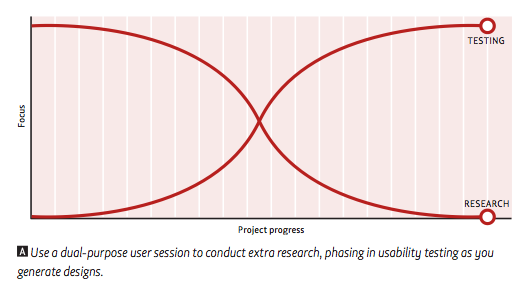
\includegraphics[width=0.6\linewidth]{images/bowles_dualpurpose_testing.png}}
  \end{center}
  \caption{User session focus chart published in ``Undercover User Experience Design'' \cite{bowles2011undercover}}
  \label{bowles_dualpurpose_chart}
\end{figure}

The first user interviews (discussed in more detail in the following
subsections) consisted mostly of research; for example, discussing how module
allocation has worked in previous years. With this knowledge, a prototype
could be created. The later user sessions focused more on testing the
prototype with users to refine it and improve the user experience.

Screenshots of the three prototypes of the student interface used in testing
are given in Appendix~\ref{sec:prototypes}.

\subsubsection{With students}

In the meetings with students, the questions asked predominantly revolved
around module allocation at the University of York; it was important to
understand how students feel about the current state of module allocation to
ensure that this system improves their experience.

Students were asked to use a mockup of the application written in \gls{html}
and the researcher observed them to discover the main sources of difficulty.
Students were asked how and where they access to web, to get an understanding
of the environments this application might be used in.

During the implementation phase of the project, focus groups organised by the
\gls{aso} were conducted with students from each of the pilot departments.
\gls{lc} discussed with the students their current understanding of module
allocation, and their feelings on where it worked well and how it could be
improved. The project implementer tested several mockups of the student
interface by asking the students to visit hyperlinks. After the students had
the chance to use the mockups in a University computer classroom, they were
provided refreshments and took part in a discussion to gather their feedback.

In the History student focus group (eight students from 1st to 3rd year), it
was immediately clear that the two-column drag-and-drop layout
(Figure~\ref{prototype_student_2col}) was the easiest to use and related to
students' existing mental model most closely. As one student at the focus
group commented, this interface closely resembles the way in which the
\gls{yusu} website allows students to vote for sabbatical officers during
their annual elections. As students will already have some (however minimal)
experience with this kind of interface it makes sense to reuse ideas they are
used to.

Students were pleased with the simple drag-and-drop single column prototype,
but preferred the more explicit action of dragging from one side of the page
to the other. The weighting based system (dragging horizontal bars) was
unpopular with the History students; they commented that it would be
advantageous to have a simple system that all students can understand easily,
rather than one which may cause confusion -- especially when students are
preoccupied with making their module choices and do not want to think about
the way in which the system works.

In the Archaeology student focus group (six students from 1st to 3rd year),
similar concerns were raised about the second mockup. The students wondered
how the system would react if a only one or two modules were weighted
incredibly heavily and the remaining modules equally lightly. This is a
concern that would have to be discussed with the departments in depth and
communicated clearly to students in order to come up with an allocation that
was understood by all.

The students again commented on the similarity between the \gls{yusu} website
and the second mockup, reinforcing the previous group's feedback that this
mockup was the best of the three.

With this group of students, it was easy to observe a common issue of running
focus groups. Two of the Archaeology students present were more quiet than the
others in the group and it was harder to get their opinions. The solution in
this case was to direct specific questions at those two students, though
obviously this was not ideal. If running the session again, it would be
advantageous to not include those students in the focus group and instead
gather their opinions without the other students present.

\subsubsection{With staff}

Information was gathered from staff at the project steering group meetings and
at individual consultation sessions with each of the pilot departments.

It was mentioned at the first group meeting that previous systems used by
departments had been far too complicated for what departments required. A
departmental administrator commented that simplicity would be far more useful.

Staff raised the issue of what would happen to students who did not bother to
use the system to indicate a preference. It was decided that these students
could be randomly allocated, but that departments should be made aware which
students had been randomly allocated so that they could verify the
allocations. Related to this, departments required that they were able to send
out reminder emails to students who had not used the software.

More specific requirements started to come to light from mid-October, as staff
began to think more about the software and discuss it with colleagues.
\gls{sa} requested that some form of capability for human intervention should
be included in the software, to allow the departments to improve the allocation
once it had been made automatically.

On the issue of fairness, both departments were able to quantify their
allocation successes in previous years by saying ``no student was allocated a
module which was below their $n^{th}$ choice'' (where $n$ is different for
each department). The only other information obtained was that it would be
beneficial to keep the tail of students shorter -- that is, the software should attempt
to minimise the number of students who receive very bad allocations, if
possible.

I met with \gls{mh}, a member of \gls{ssdt}, to ascertain the format that
departments would provide the data to make the \gls{sits} import as easy as
possible. It quickly became apparent that a table in which each row was a
single allocation (a \studmod pair) would allow the team to import the data
easily. It was agreed that the following information would be provided for
each allocation:

\begin{itemize}
  \item Student information: University username, \gls{routecode}, \gls{stage}
  \item Module information: module code, number of credits, which term the module is running in
\end{itemize}

Other information was added to accompany the data as it is being imported, but it
consisted of simply static values and was purely for convenience (such as the
letter \texttt{O} to indicate optional).



%!TEX root = ../Project.tex

\subsection{Database structure}

As relational databases are so popular and are supported in many of the
software frameworks we look at in Section~\ref{sec:webframeworks}, there is no
advantage to choosing a database model apart from relational.

Web frameworks abstract away anything related to a specific database product
using an \gls{orm}, so the module allocation application can be written
without regard for the final database product that \gls{itservices} will use
to deploy the application.

Preliminary conversations with departments revealed additional requirements
for the system which informed the database structure. There are several
related entities stored by the University outside of this system, which have
the following properties:

\begin{tabular}{ l l }
  Student    & Username (unique), \gls{routecode}, \gls{stage} \\
  Module     & Module code (unique), module name, number of credits, maximum class size \\
\end{tabular}

Each module is given a number of credits representing the estimated workload
for that module, and each student must take 120 credits every academic year.

The two pilot departments currently use paper forms, copies of which are given
in [@todo Appendix~ xx]. In order to create a scalable system that could be
used across any number of departments, the project author first generalised
the paper forms provided by the pilot departments.

This generalisation involved the following observations:

\begin{itemize}
  \item Each degree type (single subject, joint honours, etc) receives a different form
  \item Each form contains one or more groups, each of which contains one or more modules
\end{itemize}

\subsubsection{Entity-relationship diagram}

Figure~\ref{er_diagram} is an entity-relationship diagram of the module
allocation system.

\usetikzlibrary{positioning}
\tikzstyle{every relationship} = [draw=black, fill=black!10, text=black]
\begin{landscape}
\begin{figure}
  \begin{tikzpicture}[node distance=8em]
    
    \node[entity] (student) {Student};
      \node[attribute] (studentid) [above=1cm of student] {\key{Identifier}} edge (student);
      \node[attribute] (routecode) [above left=1cm of student] {Route code} edge (student);
    
    \node[relationship] (makes) [below left of=student] {Makes} edge (student);
    
    \node[entity] (choice) [below of=makes] {Choice} edge (makes);
      \node[attribute] (rank) [left=1cm of choice] {Rank} edge (choice);
    
    \node[relationship] (given) [below right of=student] {Given} edge (student);
    
    \node[entity] (allocation) [below of=given] {Allocation} edge (given);
    
    \node[relationship] (allocof) [below of=allocation] {Of} edge (allocation);
    \node[relationship] (choiceof) [below of=choice] {Of} edge (choice);
    
    \node[entity] (moduleav) [below left of=allocof] {Module Availability};
      \node[attribute] (studentmin) [below left=0cm and 1cm of moduleav] {Student min} edge (moduleav);
      \node[attribute] (studentcap) [below left=1.2cm and 1cm of moduleav] {Student cap} edge (moduleav);

    \draw[link] (choiceof) |- node [pos=0.05, auto, swap] {} (moduleav);
    \draw[link] (allocof) |- node [pos=0.05, auto, swap] {} (moduleav);

  \end{tikzpicture}
  \caption{(Incomplete) Entity-relationship diagram for the module allocation system.}
  \label{er_diagram}
\end{figure}
\end{landscape}

% Helpful demo/test document

% \begin{landscape}
% \tikzstyle{every entity} = [top color=white, bottom color=blue!30, draw=blue!50!black!100]
% \tikzstyle{every attribute} = [top color=white, bottom color=yellow!20, draw=yellow, node distance=1cm]
% \begin{tikzpicture}[node distance=1.5cm, every edge/.style={link}]
%   \node[entity] (emp) {Employee};
%   \node[isa] (isa) [below=1cm of emp] {ISA} edge (emp);
%   \node[entity] (mec) [below left=1cm of isa] {Mechanic} edge (isa);
%   \node[entity] (sal) [below right=1cm of isa] {Salesman} edge (isa);      %%%%%%%%%%
%   \node[relationship] (does) [left=of mec] {Does} edge (mec);
%   \node[weak entity] (rep) [below=of does] {RepairJob} edge (does);
%   \node[ident relationship] (reps) [below=of rep] {Repairs} edge [total] (rep);
%   \node[entity] (car) [right=of reps] {Car} edge [<-] (reps);
%   \node[relationship] (buy) [below=of sal] {Buys};                         %%%%%%%%%%
%   \node[relationship] (sel) [right=of buy] {Sells};                        %%%%%%%%%%
%   % \node[derived attribute] (sval) [right=of sel] {Value} edge (sel);
%   \draw[link] (car.10) -| (buy) (buy) edge (sal);
%   \draw[link] (car.-10) -| (sel) (sel) |- (sal);
%   \node[entity] (cli) [below right=0.5cm and 3.7cm of car] {Client};
%   % \node[multi attribute] (cphone) [below right=of cli] {Phone} edge (cli);
%   \draw[link] (cli.70) |- node [pos=0.05, auto, swap] {buyer} (sel);
%   \draw[link] (cli.110) |- node [pos=0.05, auto] {seller} (buy);
% \end{tikzpicture}
% \end{landscape}



\subsection{Web application frameworks}
\label{sec:webframeworks}

% Justifying a framework for this project

While it is possible to build a web application without using a framework,
there is no advantage to rewriting basic operations for this project. If the
system needed to operate at a scale or speed far beyond what these frameworks
were capable of, it is likely that the software would have to be built from
scratch to meet those requirements.

With the limited amount of time allocated to development and implementation,
it is sensible to spend a small amount of time choosing a framework to allow
more time to implement the system.

%   Could reference the Gantt chart (if it's included) here.

\subsubsection{Framework language}

% The programming language

The most important consideration when choosing a framework is the language it
is written in, as this defines, among other things, how easy the software will
be to maintain in the future.

% ColdFusion ML
%   - http://www.york.ac.uk/communications/websites/content/programming/cms-integration/
% Java
% PHP
%   - http://www.york.ac.uk/it-services/facilities/web/php/

There are three languages used for most web development at the University of
York. \emph{ColdFusion Markup Language} (CFML) is a language for creating web pages,
the most popular commercial implementation of which is Adobe ColdFusion.
ColdFusion is used widely across the University, including in applications
such as the ``People Directory'' search tool (shown in
Figure~\ref{yorkacuk_directory_search}) and online account management
facilities. \emph{Java} was used in the creation of the new Student Portal. A
\emph{PHP} service is offered by the University for users to deploy their PHP
applications.

\begin{lstlisting}[language=HTML]
<cfparam name="attributes.userid" type="string" default="unknown">
<h1>Hello, world</h1>
<cfoutput>
  <p>Welcome, #HTMLEditFormat(attributes.userid)#.</p>
</cfoutput>
\end{lstlisting}

In a presentation at \gls{oscon} in 2007 \cite{raible2007javawebframeworks},
Matt Raible compared several web frameworks written in Java; JavaServer Faces
(JSF), Spring MVC, Stripes, Struts 2, Tapestry and Wicket.

While there are a wide variety of Java web application frameworks available,
the University of York has decided to use Spring, an open source framework
developed by a division of VMware (a virtualisation software provider). The
Spring framework has a \gls{mvc} component, making it entirely suitable for
this project. As this is a framework \gls{itservices} has deployed and can
support, it makes little sense to choose anything else.

CFML is unsuitable for this project as it is primarily a markup language -- the
allocation logic behind the application would have to be implemented in a
programming language such as Java or Python. Using two languages to create
this application would needlessly increase the complexity of any maintenance.

% Ruby
% Python

Outside the University of York, popular web programming languages include
\emph{Ruby} and \emph{Python}.

% Rails guesses the model's attributes based on the database schema, whereas
% Django requires that the model's attributes be listed in the application, and
% the schema is then created.
% 
% There's a good comparison of Django and Rails which is quite methodical. In
% it, the authors note that equivalent applications took $\frac{2}{3}$ the time
% to be implemented in Django than Rails \cite{RailsDjangoComparison_2007}.
% 
% There's also a good comparison of the three big players that pretty much rules
% out CakePHP as being rubbish \cite{EvalWebDevFrameworks_2009}.

\subsubsection{Summary}

The framework chosen for this project was Spring 3, written in Java. As the
application will be maintained by Java developers, it would not be sensible to
implement the software in another language only to possibly have to
re-implement using a different technology stack in the future.

Ruby or Python are both good languages for web application development, but
neither is suitable for this project as they cannot be maintained by
\gls{itservices}.

\subsection{Supporting software}

In addition to the web framework, there is a range of other software available
to support the creation of the application.

\subsubsection{Spring Roo}

Spring Roo is a \gls{rad} tool created by SpringSource (the Spring development team) to
aid developers in creating Java web applications. It works by providing an
executable, \texttt{roo}, which generates ``application scaffolding''
programmatically.

For example, inside Roo it is possible to run:

\begin{lstlisting}
project --topLevelPackage uk.ac.york.module_allocation
persistence setup --database MYSQL --provider HIBERNATE
entity --class ~.domain.Student
field string --fieldName username
\end{lstlisting}

These four lines of code generate a Java class representing a student complete
with setters and getters, 500 lines of XML configuration files and 20 lines of
application property files. It is also possible to generate a simple
\gls{crud} interface for displaying in the browser using the \texttt{web mvc
scaffold} command.

It is possible to tell from a brief glance that the code generated by Roo is
not as perfect as that which could be crafted by an expert Java developer. As
might be expected from a code generation tool, there is some unnecessary
repetition. The large amount of code generated results in a codebase that
feels fairly bloated, but the advantage is an application that is set up in
moments. As the generation tool is written by the Spring developers, one can
be assured that the code generated conforms to the basic standards of Spring.

The major concern when considering a generation tool such as Roo is the
lock-in that it entails. However, Chapter 6 of the Roo reference documentation
\cite{RooReferenceDocs2011} is titled ``Removing Roo''. In it, the authors
note that a key part of the Roo mission statement was ``without compromising
engineering integrity or flexibility''. The developers provide a simple,
three-step guide to removing Roo from the project. If the future maintainers
of this software require that it not include Roo, it will be easy to remove.

The benefits that Roo provides in the short-term far outweigh the time that
might need to be spent removing it.

\subsubsection{Templating engines}

% Additionally: iText PDF, JExcel, Jasper Reports, and XSLT are all supported
% by Spring

There are many different templating engines that can be used as components of
a Java (in this case, Spring) project. Examples of commonly-used Java
templating software include \gls{jsp}, Tiles and Freemarker.

% Plain old JSP

\gls{jsp} is a common language that is also used in Tiles. \gls{jsp} can be
used at a basic level to include dynamic elements in \gls{html}. The following
is an example of a \texttt{.jsp} file that outputs \gls{html} to the client:

\begin{lstlisting}[language=HTML]
<html>
  <h1>Welcome to the module allocation system, ${student_name}!</h1>
</html>
\end{lstlisting}

% Apache Tiles

Apache Tiles builds on just using \gls{jsp} markup by itself, by providing
other useful functions. Templates are written in the same language, but
developers can define `fragments' which are assembled when the page is
requested. The fragments (or tiles, which is where the software gets its name)
can be used to build up a page from its constituent parts. For example, it is
possible to define fragments for the page header and footer, to ensure they
are identical across every page. A template file may resemble the following,
where \texttt{header.jsp} and \texttt{footer.jsp} are files that contain the
site header and footer respectively:

\begin{lstlisting}[language=HTML]
<html>
  <tiles:insertTemplate path="/fragments/header.jsp" />
  <div id="container">
    <h1>This is the actual page content.</h1>
  </div>
  <tiles:insertTemplate path="/fragments/footer.jsp" />
</html>
\end{lstlisting}

% Freemarker

Freemarker is more complex than Tiles, but at the expense of not enforcing
complete separation between model and view:

\begin{lstlisting}[language=HTML]
<html>
  <#include "header.ftl" />
  <h1>Welcome to the module allocation system, ${student_name}!</h1>
  <p>These are the modules you have been allocated:</p>
  <ul>
  <#list modules as m>
    <li <#if m.level == "hard">class="hard"</#if>>${m.name} (${m.code})</li>
  </#list>
  </ul>
</html>
\end{lstlisting}

In his paper on enforcing separation between the model and the view, Parr
\cite{Parr2004templateengines} ranks Freemarker very poorly.

% StringTemplate

Parr has also created a templating engine, named StringTemplate, that enforces
separation of the model and the view. His paper articulates clearly why
enforcing the separation between model and view is a positive for a web
application, and his argument is convincing. As would be expected, his
templating engine is strict about applying the constraints he argues in favour
of in his paper.

% \subsubsection{Database thingys}

% EclipseLink or Hibernate

\subsection{Design decisions and visual appearance}

The application should be visually consistent with other University web
software to instill trust in the user.

The University's Web Office (part of the Communications Office) was contacted
to enquire whether the application should be branded using the standard green
banner, or as a part of the student portal.

% Following the principle of least astonishment...

% http://en.wikipedia.org/wiki/Principle_of_least_astonishment

% Include screenshots of University software:
%   https://www.york.ac.uk/it-services/facilities/account/accounts
%   https://www.cs.york.ac.uk/submit/assessment/
%   https://www.york.ac.uk/students/

One area that usability gains can be made are in relation to how the
application saves data. During one of the user research sessions, the
participant explained that while choosing optional modules during her first
year, she neglected to press that application's ``OK'' button and, unaware
that she had not submitted choices, was unable to take her preferred modules.

As an explicit ``Save'' button should be retained to reduce surprise and allow
the user to feel in control, the most sensible decision is to automatically
save user input periodically and notify users that their choices are being
saved. The submit button would save data in case of failure of the automatic
save mechanism.

\begin{landscape}
  \begin{figure}
    \begin{minipage}[b]{0.49\linewidth}
      \centering
      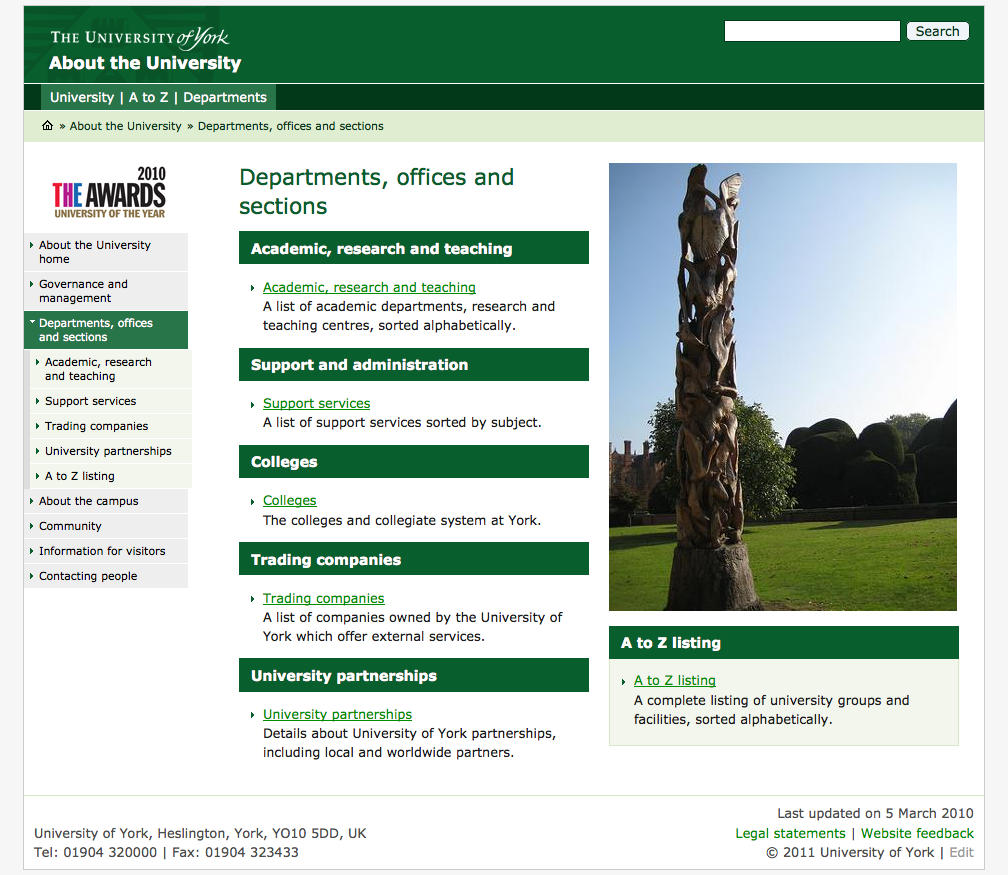
\includegraphics[width=\linewidth]{images/2011_11_06_yorkacuk.png}
      \caption{A general page on the University site, using University colours}
      \label{yorkacuk_general_page}
    \end{minipage}
    \hspace{0.5cm}
    \begin{minipage}[b]{0.48\linewidth}
      \centering
      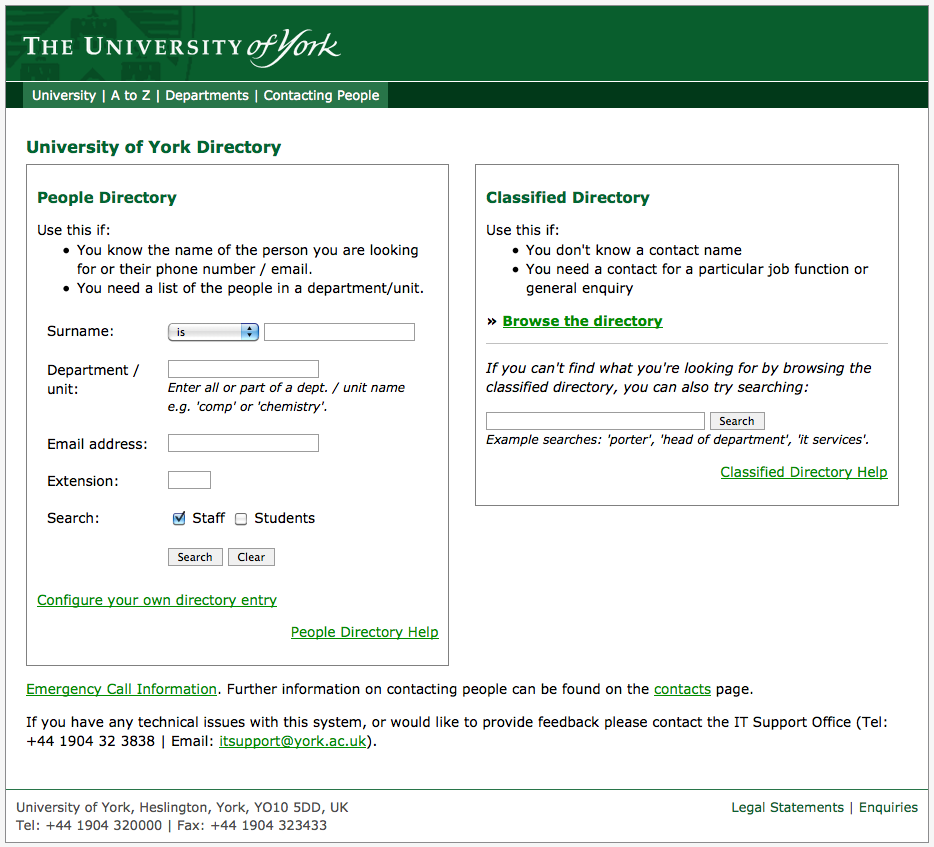
\includegraphics[width=\linewidth]{images/2011_11_06_yorkacuk_directory.png}
      \caption{The University of York People Directory search tool}
      \label{yorkacuk_directory_search}
    \end{minipage}
  \end{figure}
\end{landscape}

\subsection{Accessibility}

% http://www.york.ac.uk/communications/websites/policies/accessibility/

Educational institutions such as the University of York are required by the
\gls{senda} 2001 to ensure that web content is accessible to disabled users.
The Web Office provides advice to those publishing web sites or applications
on behalf of the University at
\url{http://www.york.ac.uk/communications/websites/content/accessibility/}.
While this advice is more applicable to content-heavy areas such as department
websites for student recruitment, it still contains some things to consider
while building a web application.

% Perceivable
% Operable
% Understandable
% Robust

The two major accessibility issues surrounding a web application are users who
are visually impaired and users who are unable to use a keyboard and/or mouse
to browse the web.

To mitigate the first accessibility issue, the application was tested to
ensure that users can increase the page or font size to fit their needs. Users
who use custom style sheets in their web browser (for example to enhance
contrast) are able to do so.

All text and background colour combinations were tested to ensure compliance
with WCAG AAA.

% http://www.snook.ca/technical/colour_contrast/colour.html

As to the second accessibility issue, generally speaking, users who are unable
to use a keyboard or mouse do not use JavaScript in their web browser. The
application is designed so that users with JavaScript disabled are instead
presented a simple form layout that can be read out to them by screen-reading
software and filled in solely with a keyboard (which can be voice controlled).

It is thought with these considerations, every student will be able to use the
system to select their modules. However, even if the above fallbacks fail the
student will still be able to obtain help from their department (which could
complete the module selection on their behalf). The aim is that no student
will be stranded with an application they cannot use and no instructions
telling them how to gain assistance.

% Finally, the student interface was tested by Mr David Swallow, a Research
% Associate in the \gls{hci} research group at the University of York. Mr
% Swallow commented that ``on the whole, the accessibility of the application
% is excellent and passes many of the checkpoints where other applications
% slip up''. He did, however, note several minor issues with the application.

\subsection{Interaction with other University software}

The system will be required to interact with \gls{sits}, as this is the
centrally maintained database that must always contain a true and accurate
representation of a student's data. Data stored in \gls{sits} is used throughout
the University, including for timetabling and room allocation.

This system will interact with data stored in \gls{sits} at two points:

\begin{enumerate}
  \item Module and student data must be imported during setup
  \item Module allocation data must be exported after the allocation algorithm has run
\end{enumerate}

The import and setup will be performed by departmental administrators. This
decision was taken to reduce the amount of time required from \gls{ssdt},
especially as administrators will need to spend time tailoring the system to
their department after the import has taken place.

For the pilot of this module allocation software, the data produced by the
application will be processed manually by \gls{mh}. He will perform a ``sanity
check'' to ensure that the data generated by the application looks accurate
and will import it into \gls{sits}. If this application is evaluated
successfully and maintained centrally, it will not be feasible to import the
data manually for each department and some kind of automatic import will have
to be developed (discussed later in Section~\ref{sec:autoexport}).

%!TEX root = ../Project.tex

\subsection{Allocation algorithm}

% Writeup from the meeting with JC

% [@todo nice and modular]
% [@todo list constraints mathematically]

\subsubsection{Human aspects}
\label{sec:algo_humanaspects}

During the research period, discussions with academic and administrative staff
in both pilot departments revealed that the current method of module
allocation is not particularly complex. With several hundred students in the
History department, it is impossible for a human to do a uniformly ``fair''
job of allocating modules to students. The staff simply try their best to
allocate as many high choices as possible.

For example, the History department allocates between one and four modules to
each of their students. The administrators and academic staff recounted how,
during the allocation period, every surface in departmental offices would be
covered with sheets of paper (one per student, numbering almost one
thousand in total) on which students had ranked their modules. The departments
would attempt to perform the best allocation possible, though clearly they had
no way of verifying mathematically that the allocation was optimal.

With this information in hand, I began to investigate how the departments and
students saw each of the choices. This influences how what the aim of the
solver will be. One could imagine an imaginary score function that a staff
member might have in their head while allocating modules:

\begin{itemize}
  \item A first choice is perfect -- if every student received every one of
        their first choices, they could not complain about the allocation.
  \item A second or third choice is alright -- a student would not be too
        displeased to be taking their second or third choice module.
  \item A fourth or fifth choice should be avoided where possible, but is not
        a show-stopper.
  \item One would expect a student who was being made to take their sixth or
        lower choice to be fairly unhappy.
\end{itemize}

Mathematically, one could sum a score for each allocation as follows:

$$
c_1(x_1) + c_2(x_2) + c_3(x_3) ...
$$

...where $x_i$ is the number of $i^{th}$ choices that that allocation created.
The coefficient multiplied by the number of $i^{th}$ choices indicates a
penalty applied by the system -- this penalty increases depending on how
negative that choice is deemed to be.

While not particularly complex, instructing the solver to minimise this result
would maximise the number of highly ranked choices. This forms the basis for
the objective function.

Eliciting these ideas explicitly from the pilot departments was one of the
harder parts of interacting with the project clients, and in fact the final
coefficients used were not confirmed until a project group meeting on 23
February, just two weeks before the allocation was due to be performed.

The Archaeology department commented that they could not recall ever having to
give a student their fourth choice or below, as they are a fairly small
department (with less than 3\% of all York undergraduates). This means that
they normally have sufficient capacity to offer every student their first,
second or third choice.

The History department is far larger than Archaeology, and additionally
reserves a number of spaces on their modules for visiting students. This will
place a strain on the allocation, as the department anticipates there will
most likely not be enough space on the most popular modules for every student
that wants to take them. History aim to give their students ``two from five''
-- that is to say, for a student ranking a group of eight modules, the two
that they will take were among their top five choices.

The final coefficients used in the objective function were decided with the
help of the departments and are shown in Figure~\ref{gurobi_coeff}.

\subsubsection{Hard constraints and pseudocode}

The hard constraints on the optimisation problem are as follows:

\begin{itemize}
  \item The lower cap on a module (a module will not run with fewer than the
        required number of students)
  \item The upper cap on a module (a staff member is not able to provide the
        required quality of teaching to more than the maximum number of students)
  \item The number of credits a student must take from a particular group of
        modules (each student must have exactly the same workload as their
        peers)
\end{itemize}

As mentioned previously, the binary variables in this system are one for every
\studmod pair indicating that a student can be allocated to that
module. These variables are written as $x_{S,M}$ in this section. Several hard
constraints were placed on the allocation by the departments, and they are
detailed here.

\noindent{\textbf{Correct number of students in a module}}

Each module has a minimum and a maximum number of students that must be placed
in it to ensure that every class size is approximately the same.

Additionally, I added more binary variables -- one for each module, to
indicate whether that module was to run or not. If the minimum number of
students could not be reached for a module, this binary variable would be set
to 0 to indicate it was not running. However, if the minimum class size can be
reached the binary variable is set to 1. These variables are written as
$y_{M}$.

The first block of pseudocode indicates that the binary variable for a
\studmod pair must be less than or equal to the binary variable
for that module. That is to say, a student cannot be allocated to a module if
the module is not running. The second block declares that if a module is
running, the sum of students must be greater than the class minimum and always
must be less than the class maximum.

\begin{spacing}{1.6}
\begin{algorithmic}
\FORALL{S,M in Student, Module pairs}
  \STATE $x_{S,M} \leq y_{M}$
\ENDFOR
\FORALL{M in Modules}
  \STATE $y_{M} \times class\_min(M) \leq \displaystyle\sum x_{S,M} \leq class\_max(M)$
\ENDFOR
\end{algorithmic}
\end{spacing}

\noindent{\textbf{Correct number of credits per group per student}}

This pseudocode demonstrates the constraint that each student is allocated the
correct number of credits from each group, subject to any elective modules
they have declared they wish to take.

\begin{spacing}{1.6}
\begin{algorithmic}
\FORALL{S in Students}
  \FORALL{G in Groups}
    \IF{S can choose modules from G}
      \STATE $group\_credits(G) - elective\_credits(G,S) = \displaystyle\sum_{M \in G} x_{S,M} \times module\_credits(M)$
    \ENDIF
  \ENDFOR
\ENDFOR
\end{algorithmic}
\end{spacing}

\noindent{\textbf{Specific departmental constraints}}

The History department required one additional constraint; that two of their
modules were exclusive (i.e. no student could take both). This code
demonstrates that no student can be allocated to both the first module and the
second module.

\begin{spacing}{1.6}
\begin{algorithmic}
\FORALL{S in Students}
  \STATE $x_{S,Module1} + x_{S,Module2} \leq 1.0$
\ENDFOR
\end{algorithmic}
\end{spacing}

\noindent{\textbf{Equity across students}}

This additional hard constraint was added later in the implementation process,
as departments enquired whether it would be possible to ensure that every
student received approximately the same ``goodness of allocation''. This
constraint is described as equity across students because it attempts to
ensure that the system does not give any single student an allocation that
would make them much happier than any other student.

The constraint is created under the assumption that there will always be at
least one student who receives the first choices they request.

A hard constraint is added to each student so that the sum of the ranks that
they gave to the modules they were eventually allocated is less than some
``equity cap'' that is defined by the department when the allocation is
performed.

\begin{spacing}{1.6}
\begin{algorithmic}
\FORALL{S in Students}
  \STATE $\displaystyle\sum x_{S,M} \times ranked(M) \leq equity\_cap$
\ENDFOR
\end{algorithmic}
\end{spacing}

\subsubsection{Gurobi Optimizer}

From the research in Section~\ref{sec:researchilp}, Gurobi appears the more
suitable choice of solver for this application. The allocation problem can be
implemented directly in the application using the Java interface, so it will
hopefully be more quickly understood by a University Java developer.
Additionally, it was found by Mittelmann to be faster than SCIP, though this
may not be relevant with the relatively small model sizes this application
will produce.

% Generated using R:
% points <- c(2048, 1000, 480, 235, 120, 60, 30, 15, 6, 2, 1, 1, 0, 0, 0)
% plot(points, xlab="Rank of module", ylab="Coefficient", main="Graph of coefficient against module ranks")
% lines(points)
% dev.copy(pdf, '/path/to/gurobi_coefficients.pdf')
% dev.off()

\begin{figure}
  \begin{center}
    \fbox{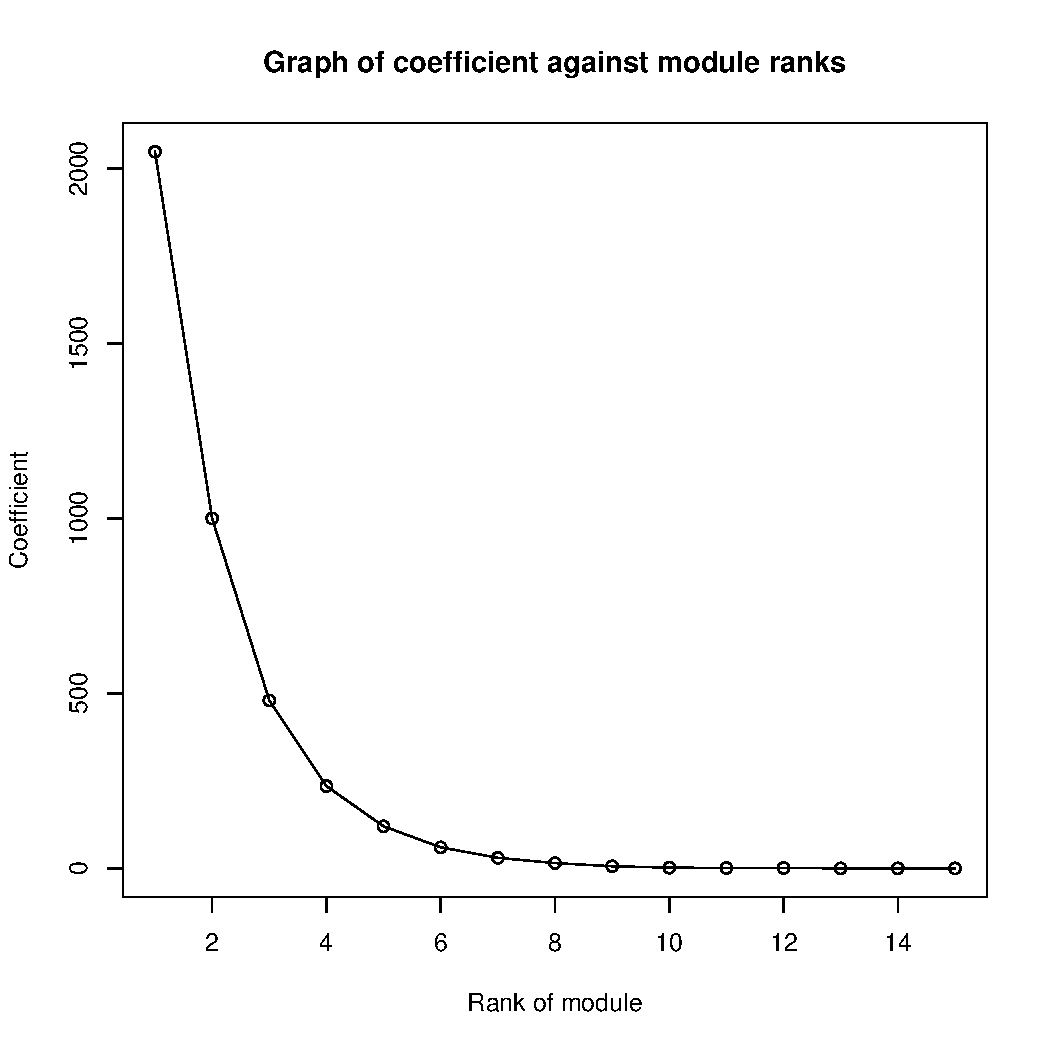
\includegraphics[width=0.6\linewidth]{images/gurobi_coefficients.pdf}}
  \end{center}
  \caption{Coefficients used in the solver's objective function}
  \label{gurobi_coeff}
\end{figure}

Figure~\ref{gurobi_coeff} shows a graph of the coefficients that were used in
the Gurobi-solved objective function. It demonstrates that the information
provided to the solver approximates the imaginary score function a staff
member might use.

To begin with, Gurobi's Python interface was used to prototype the model. As
the project implementer is more familiar with Python than with Java, it was
faster to prototype using the Python interface. Additionally, there is less
development overhead required with Python (i.e. no compilation necessary).

Once the Gurobi solver was working correctly on static data using the Python
interface, it was transferred to the application, changed to using the Java
interface and integrated with the application database.

A copy of the Gurobi code is included in Appendix~\ref{sec:gurobicode}.


%!TEX root = ../Project.tex

\subsection{Assistance provided with the application by IT Services}

\subsubsection{Development work}

An \gls{itservices} developer was provided to assist with the integration of
the project into the University's infrastructure. As the framework was chosen
so that it was familiar to the University's developers, a certain amount of
code reuse could occur between this system and other already existing
projects.

The code reuse was facilitated by this system using the same authentication
mechanism as the student portal (Section~\ref{sec:webapps_york}), another Java
application. The code to authenticate students and staff (using Spring
Security) was included into the module allocation application by the
\gls{itservices} developer.

Code for this application was committed using a \gls{dvcs} (Git) to \gls{github},
which makes it easy to see which commits came from which author.

\gls{github} provides an interface to show how much code came from each
developer. On \gls{github}, this figure is given in terms of ``impact'' (the
total number of lines of code modified, which is equivalent to lines added and
deleted). \gls{github} reports that the \gls{itservices} developer modified
336 lines of code. \mbox{``SLOCCount''} \cite{SLOCCount} (a tool for
generating statistics on source code) reports that the entire project has
2,042 Total Physical Source Lines of Code.

\subsubsection{Infrastructure}

\gls{itservices} provided a \gls{vm} for testing as well as another to host a
production instance of the application. They also provided an Oracle database.
The software was developed using a MySQL database, but as it used an
\gls{orm}, this simply required a minor configuration change so that the
application knew where to find the production database.

Finally, once the software had been deployed to the production instance, they
mapped a URL from under \texttt{www.york.ac.uk/students/} to connect students
and staff to the application.

\subsubsection{Security review}
\label{sec:securityreview}

On 15 February 2012, a review of the application architecture was conducted by
the University's Information Security Officer and the developer mentioned
previously who assisted with integrating the application's security
configuration.

As well as being targeted at departments, the software documentation created
by the project author also describes possible security vulnerabilities and how
they were mitigated. This documentation is provided in
Appendix~\ref{sec:documentation} and was given to those present at the
security review meeting.

The web hosting configuration and application security model was reviewed. Two
recommendations were made about the code; primarily, that the application
should use the \gls{owasp} ESAPI library for escaping special characters to
prevent some attacks noted in Section~\ref{sec:research_security}.

The security expert considered that the data held by the system could be
classed as between medium and low risk, as there was no highly sensitive
personal information such as student telephone numbers or email addresses.


%!TEX root = ../Project.tex

\subsection{Issues arising during implementation}
\label{sec:issuesarising}

% Discuss some of the _real_ issues of a _real_ project

\noindent{\textbf{Availability of stakeholders}}

One of the most positive aspects of undertaking this project was in fact one
of the most difficult -- that is, the project was designed to work very
closely with the University of York and as such relied on ``real''
stakeholders.

An issue arose fairly early in the project when it became clear that some
administrative staff (both IT support staff and those in the pilot
departments) would be away from work for prolonged periods of time or would
leaving their jobs during the creation of this application. This caused delays
while the replacement staff had to be brought up to speed on the background
and current state of the project.

The issue was mitigated with the help of the \gls{aso}, which was responsible
for assisting with issues not directly related to implementation. The new or
replacement staff were then invited to group meetings so that they could keep
up to speed with recent developments and provide any necessary input. As
implementation began to finish, departmental administrators were provided
training on the software by the project implementer. A deputy was present at
the training sessions so that the software could still be used in case of
unforeseen circumstances rendering the departmental administrator unable to
set up the software.

\noindent{\textbf{Lack of technical contacts available during the project}}

I first met the Head of Web Services and an \gls{itservices} developer on 16
January, several months after the project had begun, and this meant that the
amount of time allocated to implementation was reduced. If a project of this
nature was to be carried out in future, the technical contacts
(\gls{itservices} in the case of the University of York) should be involved as
early as possible. I am of the opinion that earlier involvement from a
developer would have resulted in the developer actually spending less time
assisting with the project overall.

\noindent{\textbf{Inability to interact with the system while it contained sensitive data}}

The project implementer was unable to respond to bugs in a timely manner as it
was not possible for \gls{itservices} to provide access to the database and
logs for an application containing live student data. This made bug fixing in
the live environment nearly impossible.

Specific bugs that occurred during the pilot are described later, in
Section~\ref{sec:developmentpilot}. Generally, the process surrounding bug fixing
was as follows:

\begin{enumerate}
  \item An error is reported by a departmental administrator
  \item The administrator contacts \gls{itservices} and/or the project implementer
  \item They liaise (in order to provide redacted log files, if necessary)
  \item The software is patched by the project implementer
  \item The patched software is deployed by \gls{itservices}
\end{enumerate}

Because of the dependency between the various different people involved in the
project, fixing a bug was a process that took several hours. While releasing a
patched application in one or two days is relatively uncommon in, for example,
desktop software development, it is a long time for a web application that is
only in use for two weeks.

The web application was only available to students for a week, or about 120
waking hours. Under the assumption that the use of the application by the 800
students was distributed uniformly over that time, a several hour period during
which the software was not fully functional might inconvenience approximately
forty students.

The project implementer signed a non-disclosure agreement in order to protect
the student data involved in the system, but ultimately it was still felt by
the University that a student could not be given access to other students'
personal data.

\noindent{\textbf{Unfamiliarity with the language and framework}}

While the framework was chosen based on its maintainability as
University-owned software, the project implementer was not particularly
familiar with the underlying language and framework. This made it hard to
estimate the amount of time that various stages of implementation would take.
If this project was to be undertaken again, the implementer should first use a
language they are familiar with to prototype the application quickly, and then
use any remaining time to re-implement in a language that can be maintained by
the future software owners.

This would require almost double the implementation effort (though parts, such
as the user experience and some front-end code, could be reused across
frameworks) but should allow the implementer to provide clients with a working
application far in advance of any deadlines. When developing using unfamiliar
software, the developer is dependent on how fast they are able to learn and
use new techniques.


%!TEX root = ../Project.tex

\subsection{Testing}

% Unit tests?
% Performance testing?

% User testing

Prior to the application being made available to students, members of staff
and students were requested to test the application. A summary of the feedback
is given in Appendix~\ref{sec:testingfeedback}.

As a result of this feedback, several changes were made in advance of the
application being made accessible to students:

\begin{itemize}
  \item The form validation was improved so that elective credit values were properly checked
  \item Modules displayed on the confirmation screen were put in ascending order of rank
  \item The explanatory text was clarified with the help of departments and the \gls{aso}
\end{itemize}

% Algorithm testing

The departments provided their finalised courses, modules and students (making
use of randomly generated ``fake'' usernames) to the project implementer. He
was then able to perform an allocation based on this data with random rankings
created by the system, to ensure that the allocation algorithm performed as
expected.

The random rankings were generated during testing using the following
pseudocode:

\begin{verbatim}
  For each student in the sytem:
    Get the student's choices and clear them
    Get the student's groups
    For each of the student's groups:
      Get the list of modules in that group
      Randomise the list
      Set rank = 1
      For each module in the randomly-ordered list:
        Assign it a value of `rank'
        rank += 1
        Create a choice entity for this (student, module, rank)
    Save the student's choices
\end{verbatim}

Clearly students do not rank modules with absolute uniform randomness in
practice. Some modules are more popular than others, and as such will receive
more first choices. This will influence the objective function, but these
random rankings were used to provide useful information on whether the hard
constraints of the model could be met.

Initially, the data provided by the History department caused the solver to
report that finding any allocation, no matter what the value of the objective
function, was an insolvable problem. In this case, Gurobi reported that the
model was infeasible.

The project implementer noted that the \gls{iis} computed by Gurobi revealed
that modules with database ID from 1 to 8 were the problem modules -- the
solver was unable to find a solution such that the maximum class size
constraint could be met for these modules. These eight modules had these
properties in the database:

\begin{verbatim}
  id   code   min   max   credits
 ---------------------------------
  1    02I    56    64    20
  2    06I    56    64    20
  3    13I    56    64    20
  4    15I    56    64    20
  5    58I    56    64    20
  6    59I    56    64    20
  7    64I    56    64    20
  8    65I    56    64    20
 ---------------------------------
\end{verbatim}

On further inspection, it was revealed these eight modules form the
department's ``Histories and Contexts'' group. They are self-contained
modules; they only appear with all eight together and never with any other
modules. This means that it is possible to count exactly the number of
allocations that will be required to be made by the system.

The following table shows the seven groups that these modules appear in. For
each of these seven groups, the departments have specified a number of credits
that the system is required to allocate. As the modules are all worth 20
credits either one or two allocations needs to be made, depending on the
group.

\begin{verbatim}
  group_id  sheet_id  credits_to_alloc  mods_to_alloc  num_students  num_allocations
 ------------------------------------------------------------------------------------
  1         1         40                40 / 20 = 2             220    220 x 2 = 440
  3         2         20                20 / 20 = 1               1      1 x 1 =   1
  5         3         20                20 / 20 = 1               6      6 x 1 =   6
  7         4         20                20 / 20 = 1              11     11 x 1 =  11
  9         5         20                20 / 20 = 1              26     26 x 1 =  26
  11        6         20                20 / 20 = 1               7      7 x 1 =   7
  13        7         40                40 / 20 = 2              16     16 x 2 =  32
 ------------------------------------------------------------------------------------
  Total:                                                        287              523
\end{verbatim}

As each group has a fixed number of students associated with it, it is trivial
to see that 523 allocations \textbf{must} be made by the system in order to
meet the hard constraint that every student takes the correct number of
credits. However, each of the eight modules was given a cap of just 64
students, meaning the solver could only ever generate 512 allocations.

The History department was consulted and it was revealed they had been overly
cautious when setting the cap to allow sufficient places for visiting
students. In fact, the cap had been set so low that there was not enough space
for each student in the department to take their full quota of modules.
Increasing the cap on these eight modules from 64 to 66 meant that 528
allocations could be made. The allocation was tested with these new caps and,
as expected, it completed without problems.

The anonymised data provided by the Archaeology department did not cause the
solver to report any problems. As discussed in
Section~\ref{sec:algo_humanaspects}, Archaeology has far more available
capacity in their modules than History so this is unsurprising.


%!TEX root = ../Project.tex

\subsection{Software overview}
\label{developmentsoftwareoverview}

This section of the report gives an overview of the feature-complete software,
including a walkthrough of the entire selection and allocation process. There
are two parts to the software; an administrative interface (used in the setup
and allocation phases) and a ranking interface (used by the students).

\subsubsection{Setup}

On loading the main administrative page, users are greeted with a form that
allows them to setup the system by uploading their ``assets'' from four
\gls{csv} files (Figure~\ref{walkthrough_admin_main}). Setup is conducted
simply by uploading these four files:

\begin{enumerate}
  \item Sheets (one for each different type of student using the system)
  \item Modules
  \item Groups (one or more per sheet)
  \item Students
\end{enumerate}

\subsubsection{Ranking}

The interface that students use to rank their modules after logging in is
shown in Figure~\ref{walkthrough_student_rank}. The user drags modules from
the left column to the right column using their mouse. For users without
JavaScript enabled in their web browser, a simple \gls{html} form appears
instead of this interface. The screen displayed to students after clicking
``Save choices'' is shown in Figure~\ref{walkthrough_student_confirm}. It
contains one table for each group visible to the student, with the modules
listed in descending order of rank.

Administrators can use the main administrative page
(Figure~\ref{walkthrough_admin_main}) to make a ranking on behalf of a student
-- after clicking ``Make a ranking on behalf of a student'', the application
prompts the administrator for a student username and then displays the
appropriate ranking interface -- identical to the one shown to students.

% A video of the software in use on a touchscreen device is available at...?

\subsubsection{Allocation and export}

Once the allocation period has ended, administrators can return to the main
screen to view all the choices made by students and to perform the allocation
and tweak the results as necessary.
Figure~\ref{walkthrough_admin_view_all_choices} is included to show the scale
of the table containing all choices -- this particular table contains the same
number of choices as were made during the History department's pilot
run\footnote{591 students and 57 modules, totalling approximately 18000
choices as every student did not have to rank every module}.
Figure~\ref{walkthrough_admin_view_all_choices_visible} is a close-up view of
the same choices table, in which every student and the ranks that they gave
their modules are shown.

There is also a table of allocations which is identically structured. The
table is blank to begin with, before allocations have been made.
Figure~\ref{walkthrough_admin_view_all_allocations_bottom} shows the bottom of
the allocations table, including the form that departments use to perform the
allocation. The text input is only relevant to the History department -- the
value entered is used as the ``equity cap'' mentioned in
Section~\ref{sec:algo_constraints}.

% Figures here:

\begin{landscape}
  \begin{figure}
    \begin{minipage}{0.5\linewidth}
      \centering
      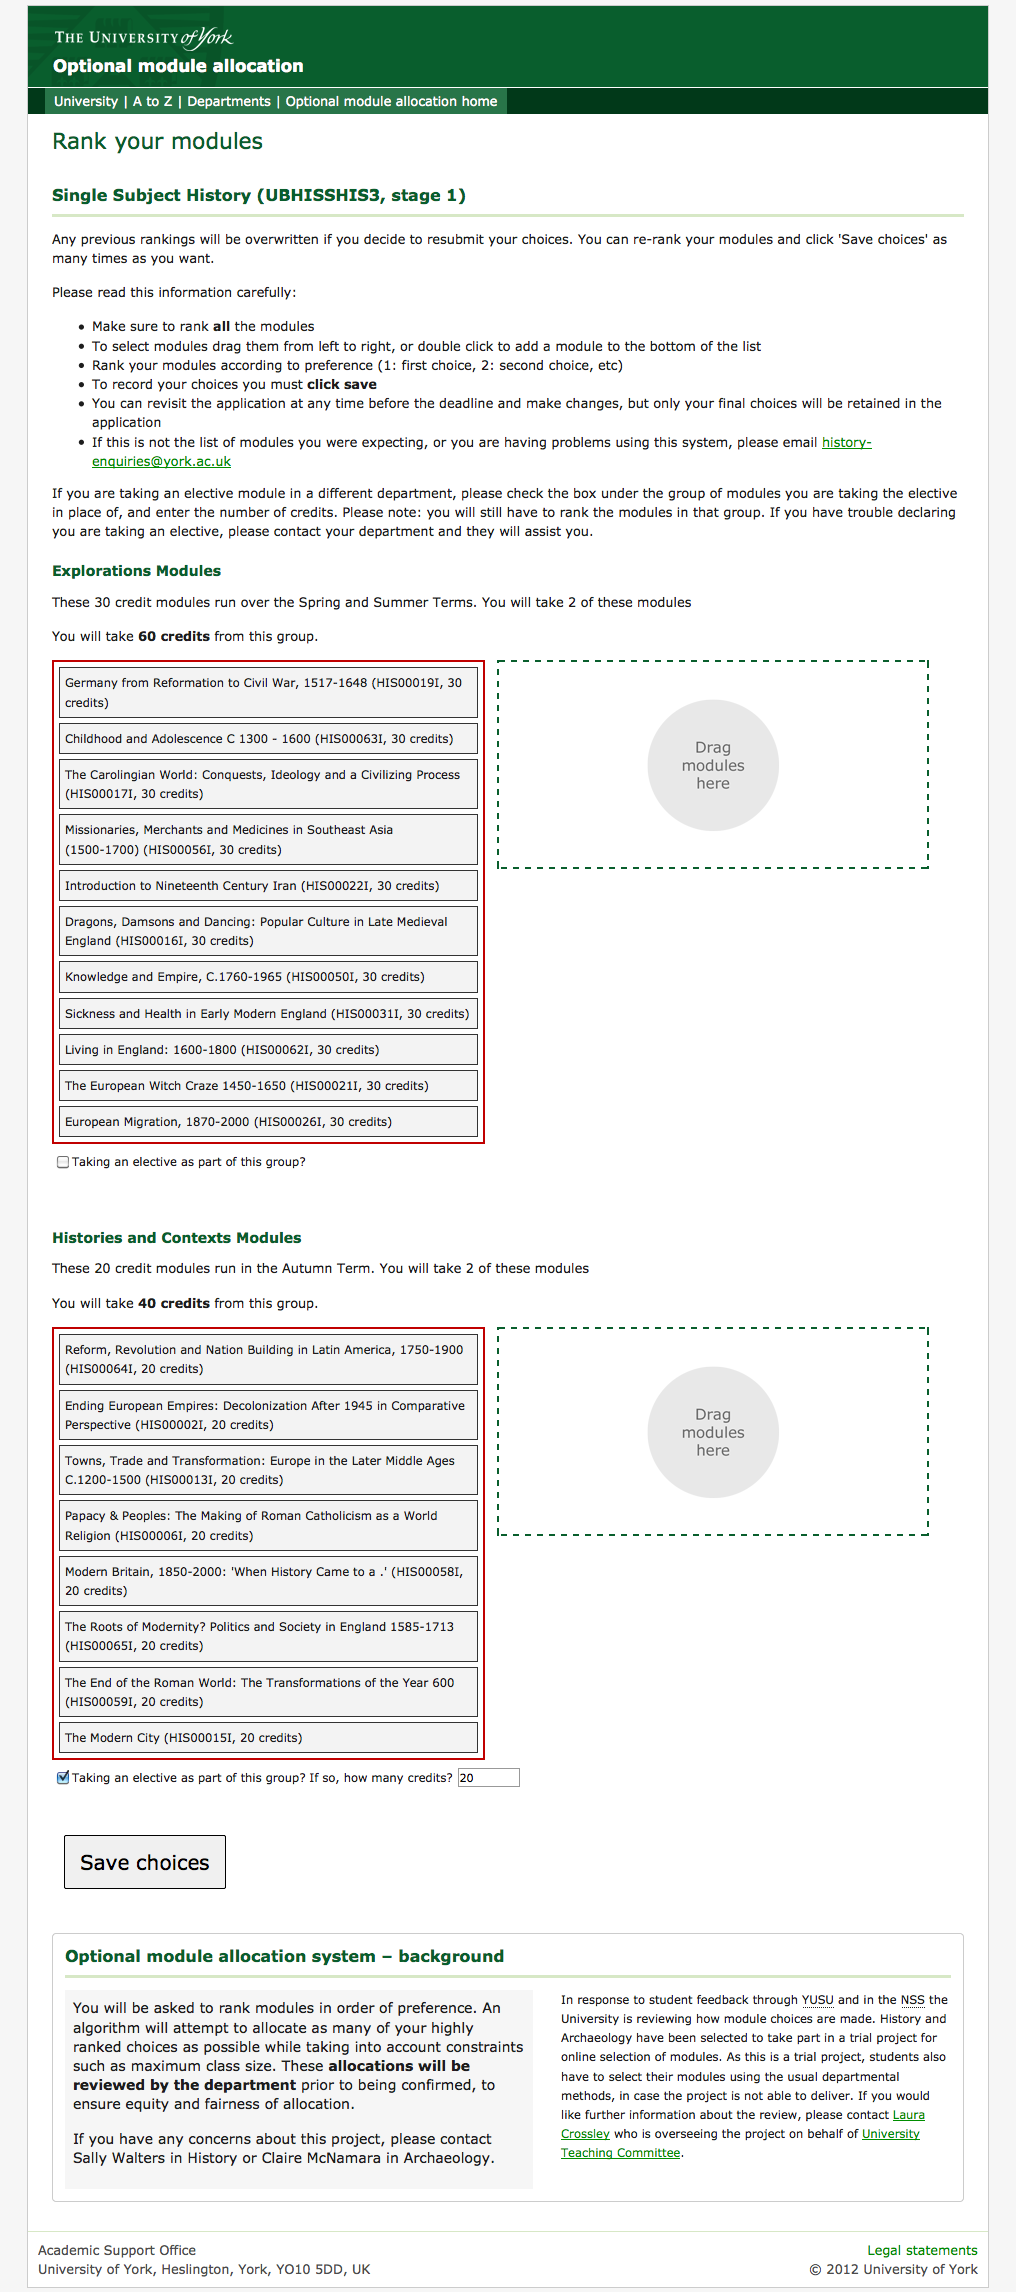
\includegraphics[width=0.6\linewidth]{images/walkthrough/student_rank_modules.png}
      \caption{The student ranking interface}
      \label{walkthrough_student_rank}
    \end{minipage}
    \begin{minipage}{0.5\linewidth}
      \centering
      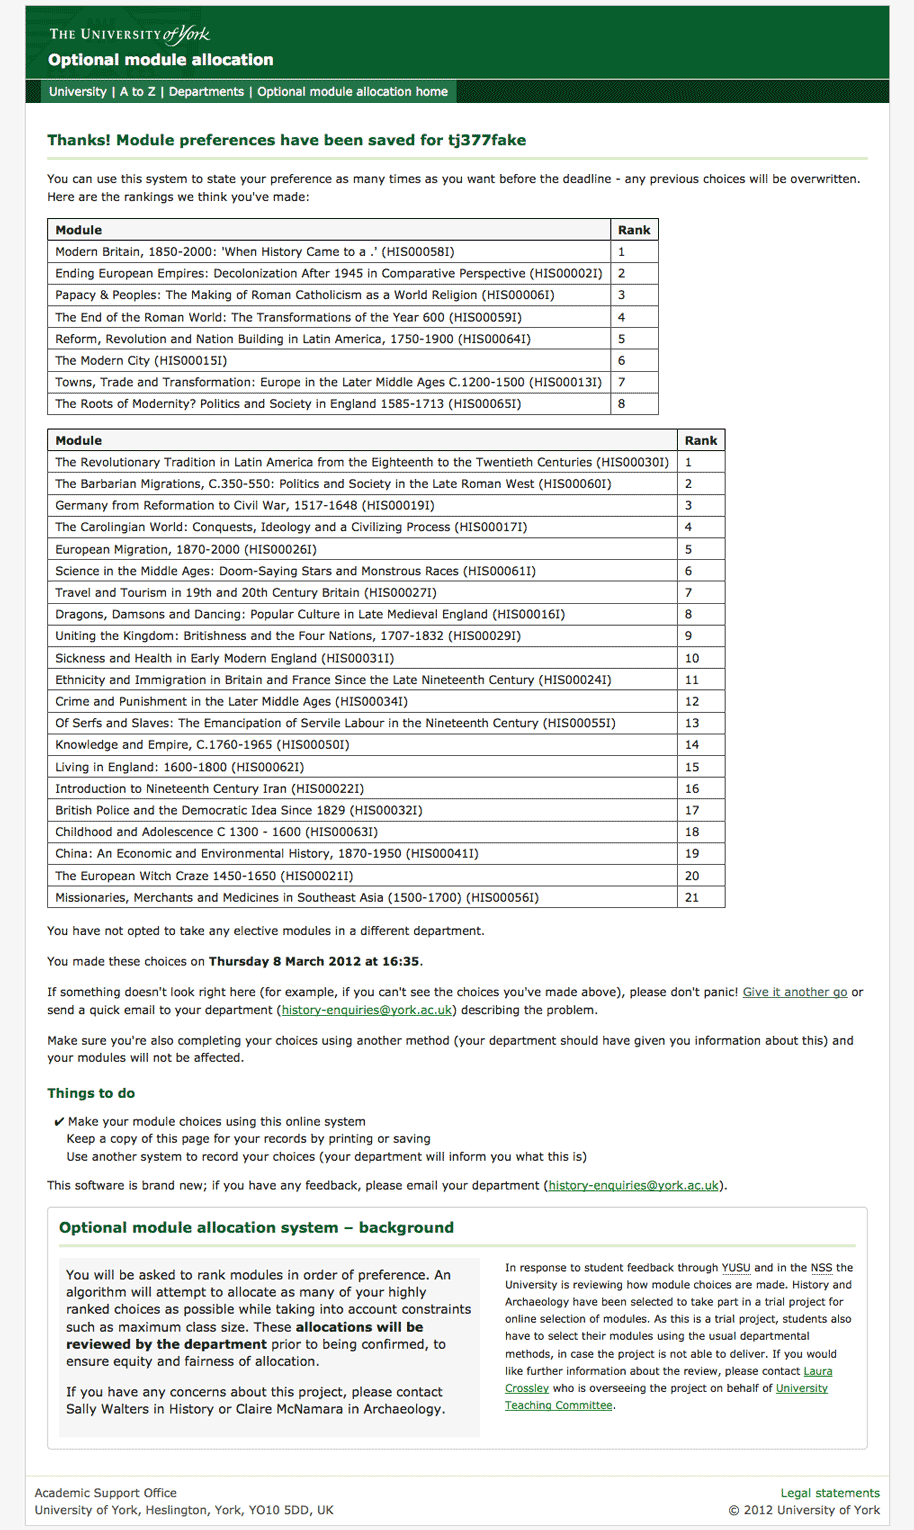
\includegraphics[width=0.8\linewidth]{images/walkthrough/student_confirm_modules.png}
      \caption{The student confirmation interface}
      \label{walkthrough_student_confirm}
    \end{minipage}
  \end{figure}
\end{landscape}

\begin{landscape}
  \begin{figure}
    \begin{minipage}{0.5\linewidth}
      \centering
      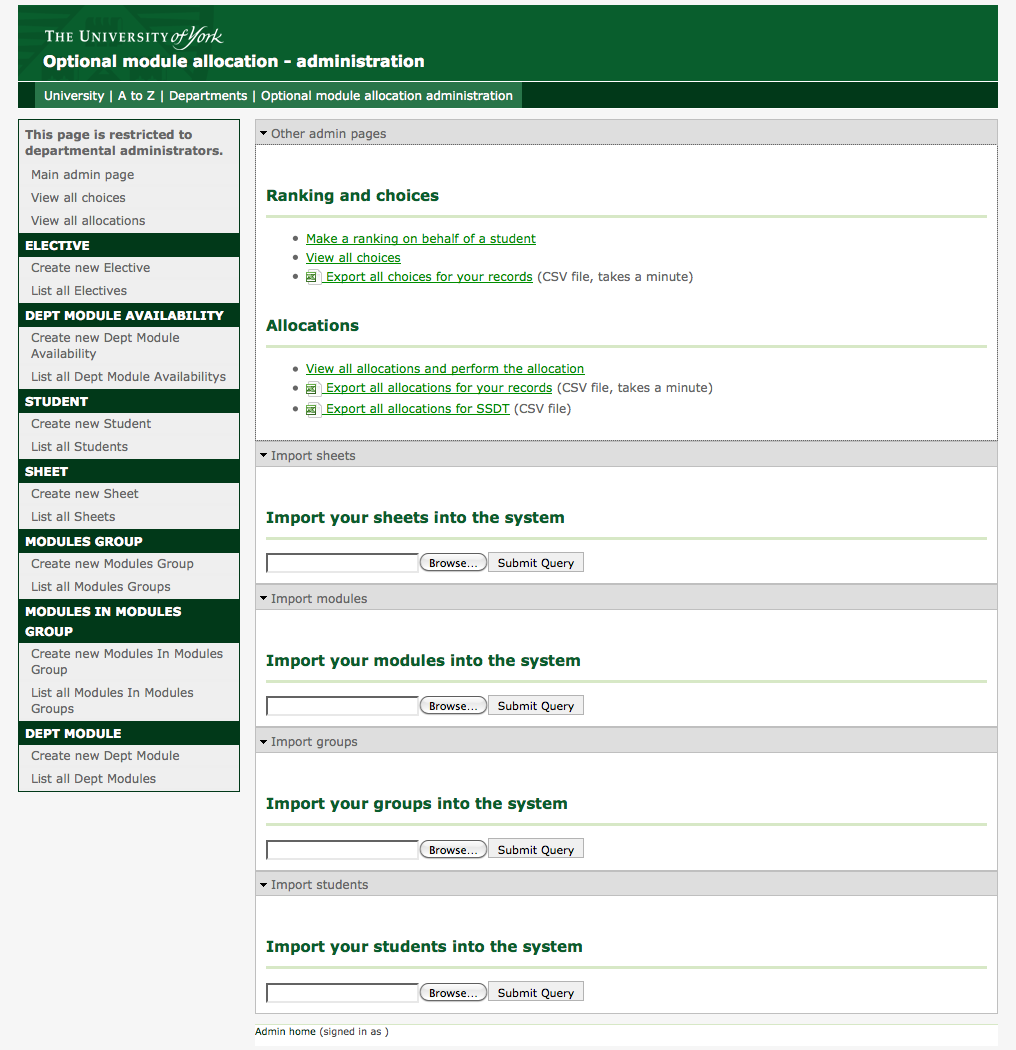
\includegraphics[width=\linewidth]{images/walkthrough/admin_main.png}
      \caption{Main administrative page of the application}
      \label{walkthrough_admin_main}
    \end{minipage}
    \hspace{0.5cm}
    \begin{minipage}{0.5\linewidth}
      \centering
      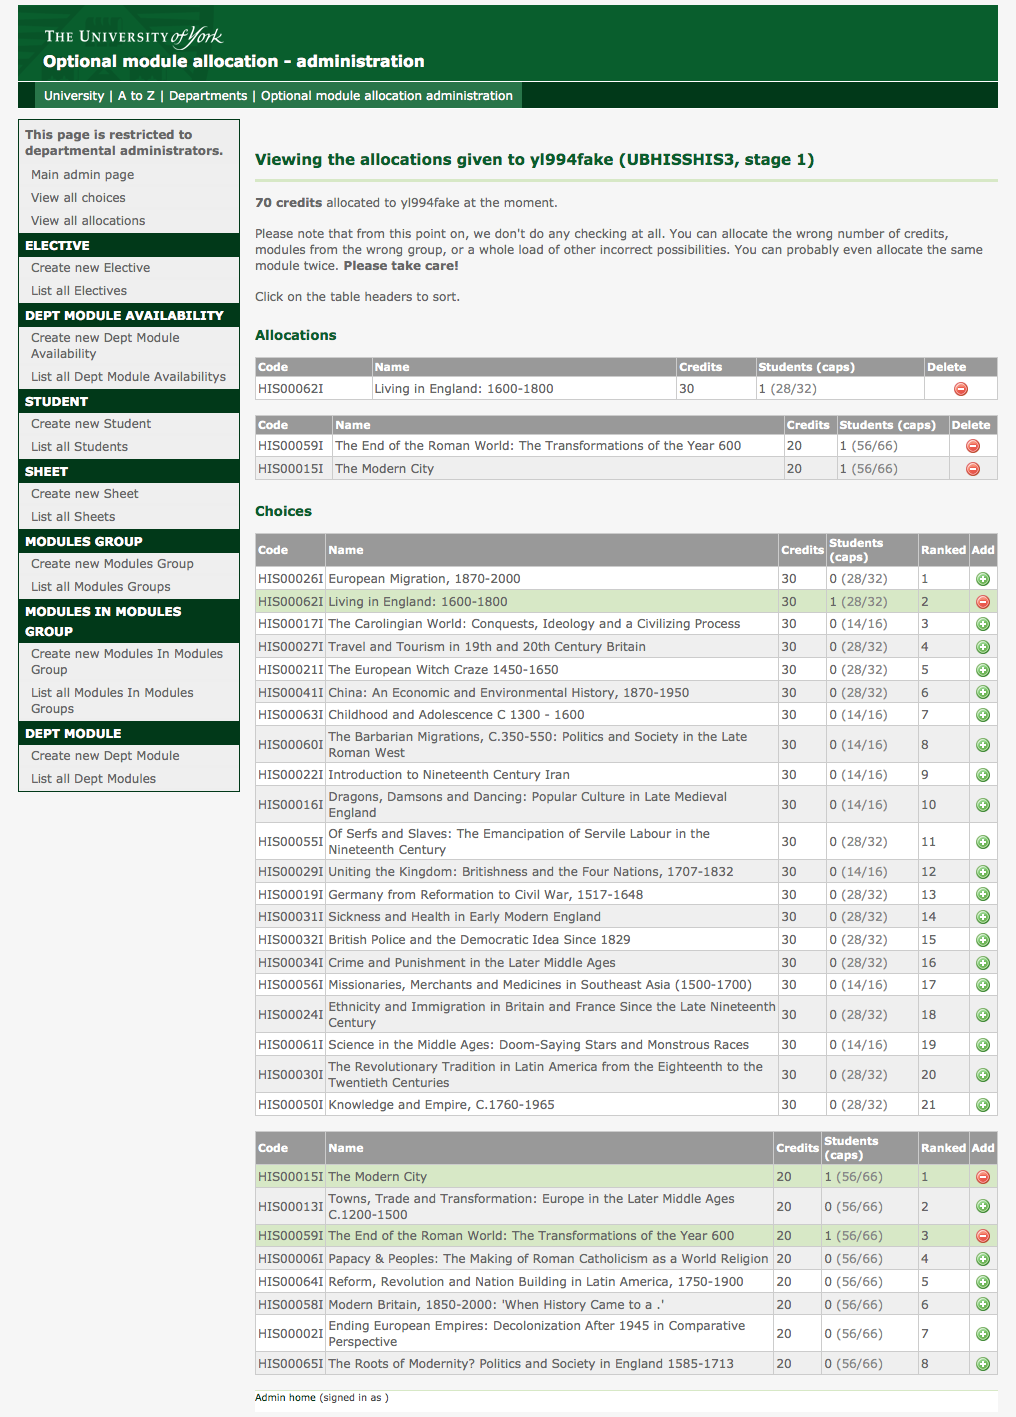
\includegraphics[width=0.9\linewidth]{images/walkthrough/admin_view_student.png}
      \caption{The tweaking view for an individual student}
      \label{walkthrough_admin_view_student}
    \end{minipage}
  \end{figure}
\end{landscape}

\begin{figure}
  \begin{minipage}[]{0.33\linewidth}
    \centering
    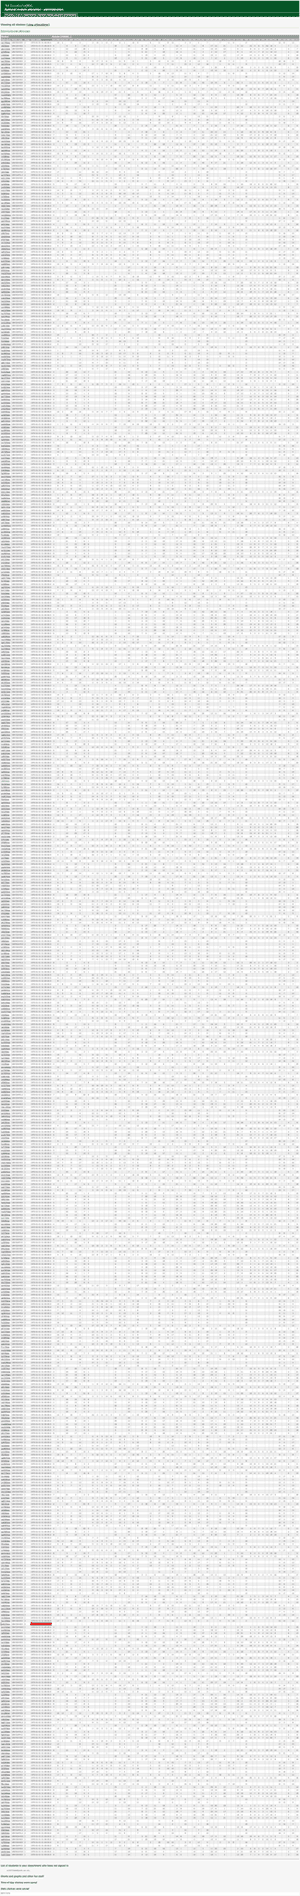
\includegraphics[width=0.6\linewidth]{images/walkthrough/admin_view_all_choices.png}
    \caption{Admin interface showing the number of choices made in the History pilot}
    \label{walkthrough_admin_view_all_choices}
  \end{minipage}
  \hspace{0.1cm}
  \begin{minipage}[]{0.63\linewidth}
    \centering
    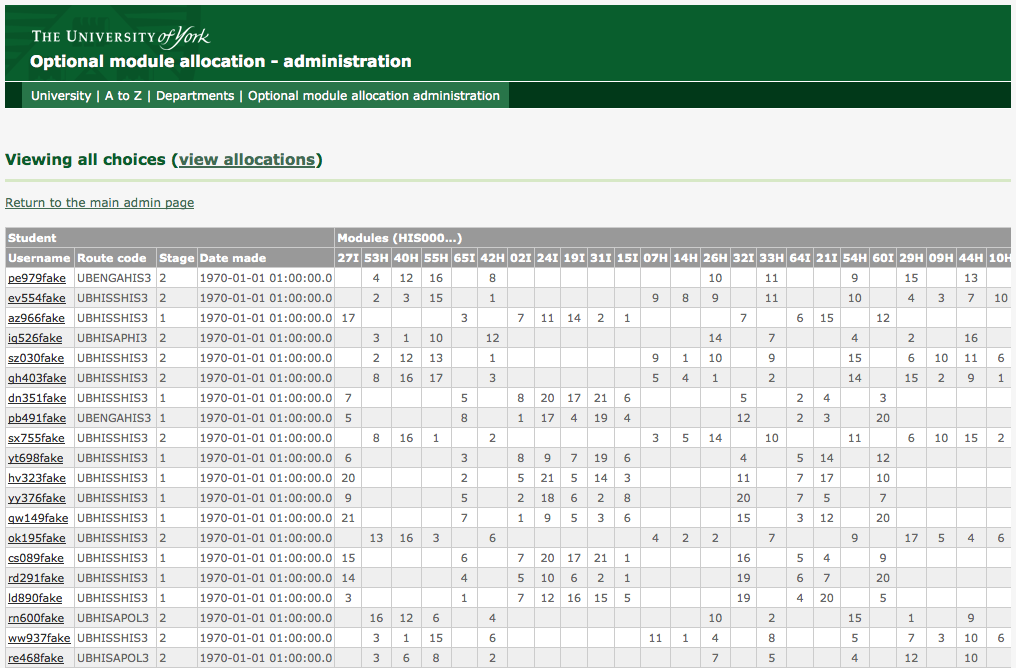
\includegraphics[width=0.9\linewidth]{images/walkthrough/admin_view_all_choices_visible.png}
    \caption{The top of the choices table}
    \label{walkthrough_admin_view_all_choices_visible}
    \bigskip
    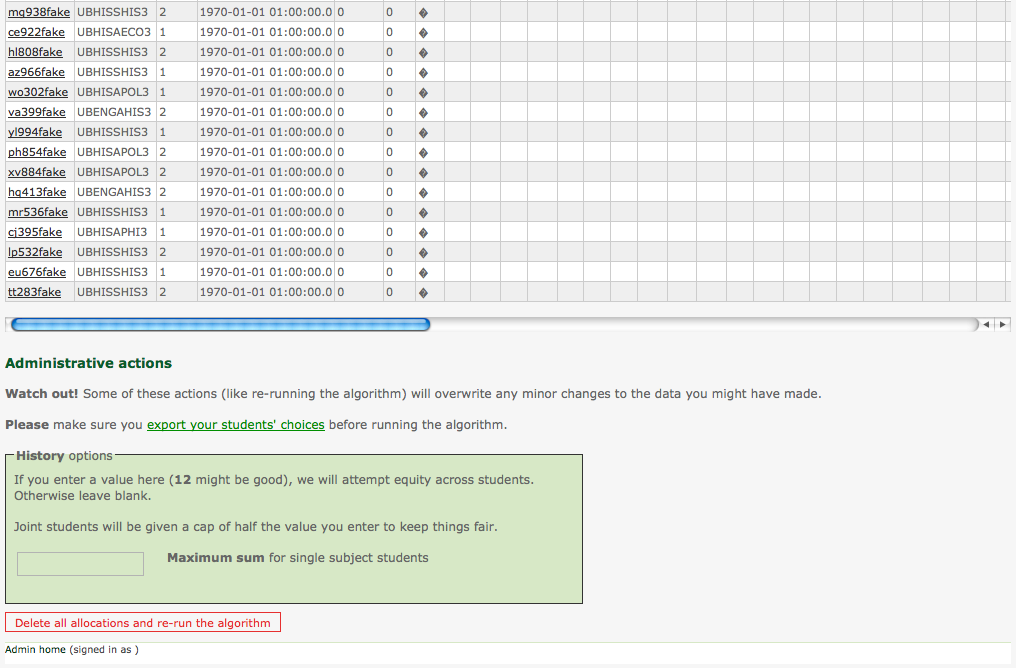
\includegraphics[width=0.9\linewidth]{images/walkthrough/admin_view_all_allocations_bottom.png}
    \caption{The bottom of the allocations table}
    \label{walkthrough_admin_view_all_allocations_bottom}
  \end{minipage}
\end{figure}

Finally, Figure~\ref{walkthrough_admin_view_student} is the tweaking
interface. Once an allocation has been performed, departments can access this
interface by clicking on a student's username. It allows them to delete and
add allocations if they decide they want to make an exception for a particular
module size. Not pictured is the ability to modify module minimum and maximum
sizes and re-run the allocation using these new constraints.

\Gls{csv} files are made available to download using the links on
Figure~\ref{walkthrough_admin_main}. The downloads available are:

\begin{itemize}
  \item A file containing all choices (a table indexed by students and modules)
  \item A file containing all allocations (again, indexed by students and modules)
  \item A list of every allocation made by the system, to be passed to \gls{ssdt}
\end{itemize}


%!TEX root = ../Project.tex

\subsection{Pilot by the Archaeology and History departments}

During the spring term (January to March 2012), the Archaeology and History
departments at the University of York used this application to allocate
modules to their second and third-year students. The application documentation
(Appendix~\ref{sec:documentation}) includes information for departmental
administrators about the setup of the application and limitations they should
be aware of.

A production instance of the application \gls{vm} was provided by
\gls{itservices} from 22 February, and the application was promoted from
\texttt{wwwtest.york.ac.uk} to \texttt{www.york.ac.uk} later that day after
final sign-off from the University's Information Security Officer. The
application was set up by departmental administrators on 23 February and the
setup was confirmed after a project group meeting that day.

Table~\ref{development_pilot_department_numbers} gives the amount of
information added to the system by the pilot departments.

\begin{table}
  \begin{center}
    \begin{tabular}{ | l | l | l | l | }
      \hline
      \textbf{Department}  & \textbf{Types of student (by degree)} & \textbf{Modules} & \textbf{Students} \\
      \hline
      History     & 14                           & 57      & 591      \\
      Archaeology & 8                            & 32      & 204      \\
      \hline
    \end{tabular}
  \end{center}
  \caption{Amount of data loaded into the application by the pilot departments}
  \label{development_pilot_department_numbers}
\end{table}

As the application was hosted by \gls{itservices} on the \texttt{york.ac.uk}
domain, notification was given to the team that provides end-user support.
Issues are logged by this team from a variety of sources, including emails to
\texttt{itsupport@york.ac.uk}, telephone calls and visits to the IT Support
office. During the trial period issues relating to this application were
forwarded to departmental administrators and the \gls{itservices} developer
assisting with the application.

The application was available to students from 0900 on Monday 27 February
until 1700 on Monday 5 March. % without interruption?

% The selection process was praised by students in the Archaeology department.
% A departmental administrator in Archaeology received the following comments:

% @todo: comments from the week

% @todo: provide details of issues raised during the week

Only one issue was raised by a user to their department during the week. The
user reported they were unable to use the drag-and-drop functionality to make
their choices. It was revealed that the user was using Internet Explorer 7, a
web browser that was superseded by Internet Explorer 8 in March 2009. As of
the writing of this report, computers provided on campus at the University of
York run IE8, as well as alternate web browsers such as Firefox and Opera (all
of which were tested for this application).

The project implementer had intended to include some text for users of old
browsers, indicating that the application had not been tested for them and
they should use an alternate browser if possible. Sites such as
\url{http://www.ie6nomore.com/} include snippets of code that demonstrate how
to achieve this. Unfortunately, for some reason this code was not committed to
the repository and did not make it into the release version of the software.

The student was advised by the departmental administrator to use a more
up-to-date web browser and successfully used a campus PC to select modules
within 24 hours of the problem initially being raised.

In all, only one student raised an issue during the week, which is equivalent
to approximately 0.13\% of all users.

On [@todo 5ish] March the software was upgraded to include alterations made
during the week, and on [@todo 6ish] March an allocation was performed by each
of the departmental administrators.

% @todo: include info on how the allocation goes

% @todo: what was the students perception of equity?


%!TEX root = ../Project.tex

\section{Further work}
\label{sec:furtherwork}

% A chapter describing possible ways in which your work could be continued or
% developed. Be imaginative but realistic.

There were many feature requests from the project steering group that I had
insufficient time to implement during the course of the project. These
requests (including their difficulty and potential implementation strategy)
are discussed in this section.

\subsection{Maintaining a history}

While considering the data protection implications mentioned in
Section~\ref{sec:dataprotection}, a popular request from the pilot departments
was that the application should retain its knowledge about a student for the
duration of their time at the University. One obvious benefit of this
improvement is that the fairness of the allocation for a given student could
be improved over the course of their academic career. For example, if a
student was given one of their lower ranked modules in the first year, the
allocation could compensate them by giving them preference over other students
for their first choice in the second year.

The University's Data Protection Officer would have to be consulted in order
to draft a suitable retention policy for this additional data. It seems that
this is data that a department might be expected to collect and reference in
the normal course of a student's career, and as such could be held in line
with the department's retention policies.

Technically speaking, this is not a particularly difficult feature to
implement. Each student can be given an average score, equivalent to the sum
of the ranks they were allocated divided by the number of modules. Then,
students with a higher average score have a greater weight given to their top
choices in the objective function. Some testing would have to be undertaken
with anonymised student choices and allocations in order to ensure that the
allocation being made was still, on the whole, fair.

\subsection{Different methods of obtaining information from students}

One mockup created during the user testing allowed students to weight their
modules rather than ranking them -- it was thought by the project steering
group that this interface (Figure~\ref{prototype_student_weighting}) would
allow students to express more clearly their preferences for certain modules
(i.e. the student could use the bars to demonstrate that they have a very
strong desire for module X, and absolutely do not want to be allocated module
Y). However, user testing revealed that students were confused about how the
values shown on the bars would be used to allocate modules. Furthermore, a
concern raised at both the project steering group meetings and by students
during testing was that a selection process this nuanced might evolve into a
``bidding war'' between students, with a particular student adding one or two
points to the values their peers had input in order to secure a module. In
summary, there was strong feedback from the test groups that the application
should in fact be kept as simple as possible -- the phrase \gls{kiss} is
sometimes used in software development. It is possible that an interface
similar to the one prototyped could be refined such that students are
comfortable using it -- the project group and implementer still believe it
could provide a ``better'' allocation for students, as the system would be
given more information on which to base the allocation. A simple solution
could perhaps be to not display the exact percentage figures to students so
that they are choosing modules based on the approximate lengths of the bars
rather than the exact values.

All aspects of the student interface must be tested in detail to ensure that
they are fully accessible to users who do not use a keyboard or mouse. These
tests should include researching possible methods for providing alternative
methods of input for users without traditional input devices.

\subsection{Automatic import and export}
\label{sec:autoexport}

The application could be extended so that it automatically accesses data
stored in the University's Data Warehouse, a centralised data store which
contains \gls{sits}. This would be far easier for an experienced University
developer to implement than for me, as I have no prior experience writing
software to integrate with the University of York's infrastructure. This
enhancement would remove the need for departments to set up the application by
uploading \gls{csv} files and, crucially, would remove the requirement that
\gls{ssdt} must import the data into \gls{sits} when the allocation is
complete. The result of this integration would be a further reduction in
administrative time required.

\subsection{Expanding the use of the application}

\gls{sa} posed the question of whether this application could be used to allow
visiting students to select their modules in future. The application has been
designed in such a way that any course, no matter what the structure, can be
added. The only blocking factor for this request is that the application
requires a University of York login to authenticate with Shibboleth. A
standalone version of the application could be created with its own
authentication mechanism, which would avoid this requirement.

\subsection{Contacting students}

During user testing, one benefit students noted compared to the paper system
is that it is significantly easier for them to keep a record of the choices
they made. Currently, the system simply advises students to print or save the
page that is displayed after they have made their choices. An improvement to
this process is that students could be emailed a copy of their choices on
submission. This would confirm to the student that their input has definitely
been saved, while also giving them a copy of their choices. Again, this
enhancement is easier for a developer who has experience sending email using
University of York infrastructure.

\subsection{Support for more complex course structures}

Several departments have complex course structures, for example where a module
in one term influences the module that must be taken in the next term. The
interface could be extended to reflect this. Some members of the pilot
departments mentioned that English is a department with more complex course
and module structure, so work should be undertaken with that department to
ensure the software is as flexible as it can be.

\subsection{Improved application code and maintainability}

As with any first version of a piece of software, there are many places in
which the application code could be improved. It is currently quite fragile,
and better error handling would dramatically improve the user experience.
Additionally, as different departments have their own requirements for the
algorithm, they would greatly appreciate being able to manipulate parameters
in the allocation code themselves, such as the coefficients used in the
objective function.

In terms of maintainability, there are several places that require
improvement. One particular example is that the coefficients used in the
objective function, if static, should not be hard-coded into the Java code
(line 43 of the file given in Appendix~\ref{sec:gurobicode}). As noted in the
previous paragraph, these coefficients should ideally be stored in the
database and should be able to be modified by the departments.

The application should undergo more rigourous testing in order to locate any
issues -- this could be done through writing more detailed unit tests than the
ones generated automatically by Spring Roo. Performance testing should be
conducted, especially if the number of students using the application in
future is significantly higher than during the pilot.

\subsection{Other minor features}

There are countless other minor features that could be implemented. For
example, the system currently records a timestamp for every student when they
save their choices. It may be interesting for the departments to be able to
see at what point during the allocation period the students are making their
choices, so graphing this information may be useful.

As noted in Section~\ref{sec:developmentpilot}, the student ranking interface
should also be improved so that on subsequent uses of the software by students
the ranking interface is already filled with the choices the student has made.
As the software is currently coded, a student might find it confusing when, on
performing a second ranking, they are greeted with an interface that appears
as though they have never used the software before.

Both departments commented that the files that they export could be better
structured. This reveals that more time should have been spent detailing the
administrative interface with departments. They requested that the \gls{csv}
files also contain module names as well as module codes, and that students
were ordered or grouped by year and by \gls{routecode}. It is worth noting
that none of these requests are technically difficult to implement, which
indicates that more time should have been spent with departments when
designing the administrative functionality.


%!TEX root = ../Project.tex

\section{Conclusions}
\label{sec:conclusions}

This section contains conclusions drawn at the end of the project, including
reviewing the research undertaken and whether it was sufficient, the
application itself, and summarises the pilot departments' use of the
application, including their feedback.

% This is similar to the abstract. The difference is that you should assume
% here that the reader of the conclusions has read the rest of the report.

% Talk about the methodology you adopted and why you chose. Make sure you
% mention what worked and what did not - explain why you think things did not
% work or could be improved - this shows learning from the experience. This
% section should be a summary of everything you have done with your personal
% comments and findings and perhaps some discussion on whether you agree with
% the references you cited.

\subsection{Research}

While the research carried out formed a strong basis for creating a web
application, the lack of time dedicated to implementation meant that some
parts of the research could not be put into practice as much as I would have
liked. Additionally it would have been beneficial to spend far more time with
the project clients and end users in order to gather more detailed
requirements and perfect the application interface.

Furthermore, it became clear during implementation that there were areas I
should have researched more thoroughly, particularly database theory. This was
not helped by my unfamiliarity with the framework and associated tools -- in
the case of the Spring framework, database tables were automatically created
from the entities defined in the application logic. Spending more time testing
and playing with this before implementation started would have increased my
understanding and could have produced a higher quality application in less
time.

Early in the research period (before implementation started) I decided to
demonstrate progress to clients by creating simple \gls{html} prototypes that
had no logic behind them. Showing these prototypes to the group may have
resulted in the non-technical stakeholders believing that implementation was
further progressed than it actually was. I would still create prototypes in
the future as I believe they are the best way to involve a client in the
development process, but I would more carefully explain that it is simply a
prototype with no application code working behind it. Fundamentally, I believe
that providing mockups and prototypes to clients throughout the research
period was hugely important in allowing them to engage with the design of the
application, and as a result produced better quality software.

\subsection{Application}

The implementation of the application should have begun earlier than it did.
The increased amount of time would have provided a higher quality product and
would have reduced the stress caused by such a time-constrained implementation
period. Requirements gathering could have been completed earlier with the help
of members of the staff in the departments and earlier involvement from
\gls{itservices} may even have reduced the total amount of time that they
spent providing input for the project.

Although there was less time available for implementation than I would have
liked, I feel I have met one the key requirements that is somewhat hard to
measure: maintainability. Code quality in places is not as good as one might
expect from a bespoke (purchased) product, but as the software is written
using a framework that University developers are familiar with, I would hope
that they would be able to understand the structure of the application and
improve the code in far less time than it would take to create a similar
application from scratch -- \gls{itservices} developers have far more
experience with creating Java web applications than I do, but the constrained
optimisation part of this project is, I believe, a hugely important piece that
might they might be unfamiliar with. The code created for this application
will give any future Java developers an understanding of Gurobi, and I look
forward to walking through this part of the code with them if they would like
to. The \gls{itservices} developer assisting with the application commented
that he could think of several other areas of University software where
knowledge of constrained optimisation and linear programming might be helpful.

As mentioned in Section~\ref{sec:issuesarising}, if undertaking a project
similar to this in the future I might first create a high-fidelity prototype
in a language I was very familiar with in order to meet the basic project
requirements. I would then look at re-implementing the application in a
language that would allow it to be maintained by other developers as required.
It would be possible to reuse certain aspects of the prototype (for example,
all of the requirements gathering and some of the front-end code), and I am of
the opinion that this second implementation would be of higher quality, as
mistakes made in the prototype would not be repeated. Whether or not this
approach is suitable would depend on the nature of the project; as the module
allocation software was fairly isolated from other systems and was a
relatively small application in all, I think this would have been a good
approach to take. There was a trade-off made between my inexperience with the
chosen software framework (and therefore the amount of time implementation
took) and the usefulness of the application to \gls{itservices}. In this case,
I believe the trade-off was beneficial to the project - I managed to create a
working---though not perfect---application, and the code will still be of some
use to the University in the future. However, one can imagine a project like
this resulting in no useful software being created. This is the reason for my
recommendation to implement twice, once using an already familiar language,
when possible.

\subsection{Pilot and feedback from departments}

These underlying issues notwithstanding, the trial of the software was a
definite success. During the week when students selected their modules very
few issues arose, and those that did were mitigated with the help of
\gls{itservices} and the departmental administrators. The application was
received positively by those students who gave feedback to the departments on
the module selection process. There were problems caused by the security
requirement that the application not be available outside the University
campus. Students who attempted to use the \gls{vpn} to access the application
were unable to, and this resulted in departmental administrators having to
input those students' choices after receiving them by email (7 out of 204 in
the case of Archaeology). This issue would require further investigation by
those with access to relevant log files to resolve.

An area I would like to have spent more time improving is the allocation
process and the associated constraints. If running this project again, I would
be more firm with eliciting allocation-related requirements from departments
earlier in the process, helping them to be decisive in quantifying soft
constraints (such as the coefficients used in the objective function). This
should be easier in future years as this pilot has provided some results which
can be iterated on with feedback from the departments.

This trial has also provided departments with data that they had never had
access to in the past -- the History department, with almost one thousand
undergraduates in total, had never before been able to analyse the choices
that students made in order to make decisions about the courses they offer.
The department felt that the data provided by this application would be
incredibly useful in allowing them to quantify the popularity of their modules
and would inform decisions about staffing and resourcing made in the future.

Unfortunately, some of the time savings that this application would have
provided were offset by time that departments had to spend during requirements
gathering and training sessions, learning to use the new software. These time
savings will be seen in future years if the software is used again. The
biggest time saving was in the software creating a \gls{csv} file of
allocations for \gls{ssdt} to process. In previous years the departmental
administrators would have to input each student's modules one by one. The
Archaeology department estimated they had saved one day's work with this file
being generated by the software, and the History department several days
because of their larger student population.

The Archaeology department commented that out of the 204 students who used
this system, just three contacted \gls{cm} to indicate they were unhappy with
the modules they had been allocated. \gls{cm} commented that she had a feeling
this was ``fewer than usual, but [that she] couldn’t back that up with
anything''. Due to the deadline for this report I am unable to provide any
student feedback on the allocation from the History department, though the
staff felt that the allocation, with some manual modifications, was as good as
they could have managed by hand.


\clearpage
\appendix

\stdsection{Participant consent form}
\label{sec:consent}

Research participants (students and staff of the University of York) signed
the consent form shown in Figure~\ref{participantconsent} before their
interview took place. This form is adapted from one made available by Alistair
Edwards for Computer Science students to use during their projects. As of 5
November 2011, the original is at
\url{http://www-users.cs.york.ac.uk/~alistair/projects/consent.html}.

In each case, the top half of the form was retained by the project author and
the second half was given to the participant in case they had any further
questions about the interview.

\stdsection{Confidentiality and non-disclosure agreement}
\label{sec:nda}

The \gls{nda} shown in Figure~\ref{confidentialitynda} was signed by the
project implementer and the Head of Web Services at the University of York.

\stdsection{Paper forms used for module selection}
\label{sec:paperforms}

Figures~\ref{paperformarchaeology1} and \ref{paperformhistory1} show
paper forms used by each of the pilot departments to allow students to rank
their modules in order of preference.

\begin{figure}
  \begin{center}
    \fbox{
\includegraphics[width=0.9\linewidth]{inc/itservices_nda.pdf}}
  \end{center}
  \caption{University of York confidentiality and non-disclosure agreement}
  \label{confidentialitynda}
\end{figure}

\begin{landscape}
  \begin{figure}
    \begin{minipage}[b]{0.48\linewidth}
      \centering
      \fbox{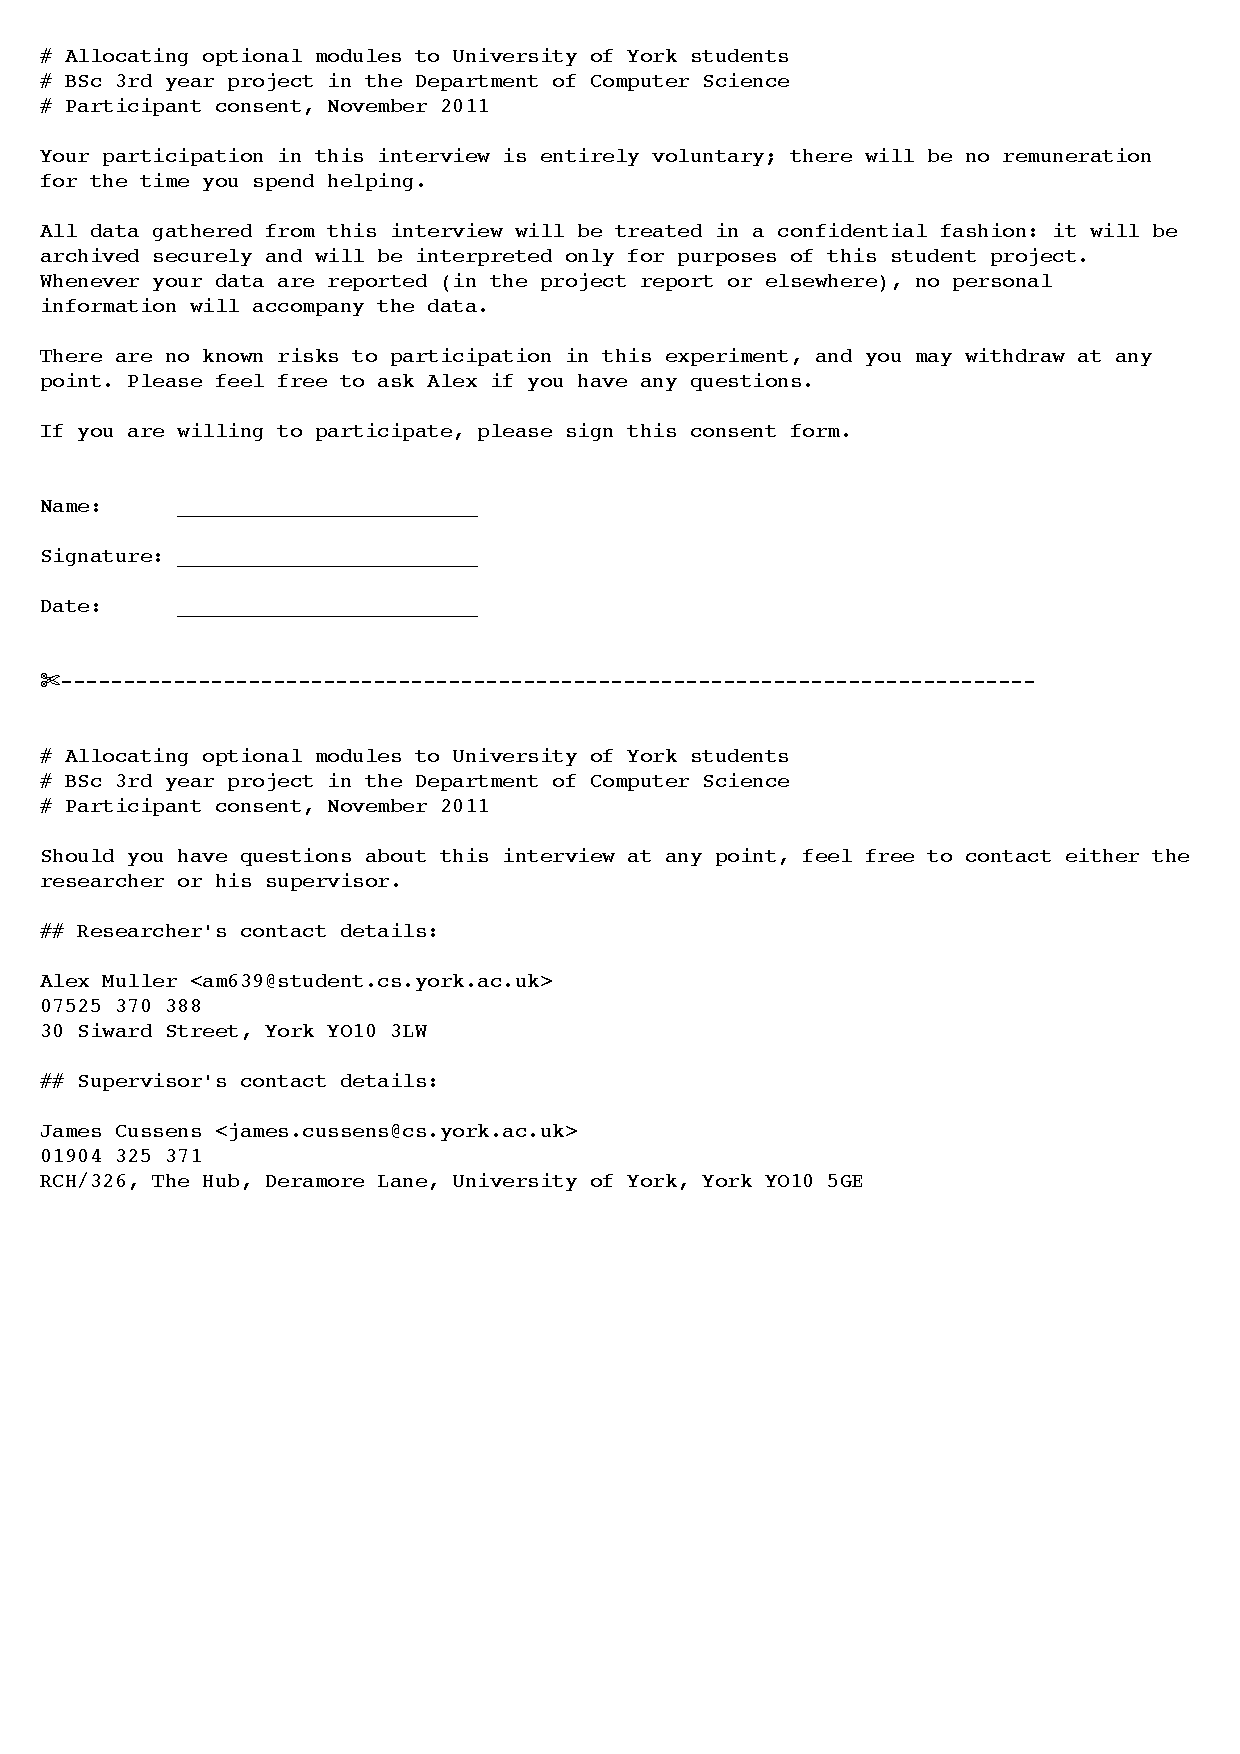
\includegraphics[width=0.9\linewidth]{images/consent.pdf}}
      \caption{Participant consent form}
      \label{participantconsent}
    \end{minipage}
    \hspace{0.5cm}
    \begin{minipage}[b]{0.49\linewidth}
      \centering
      \fbox{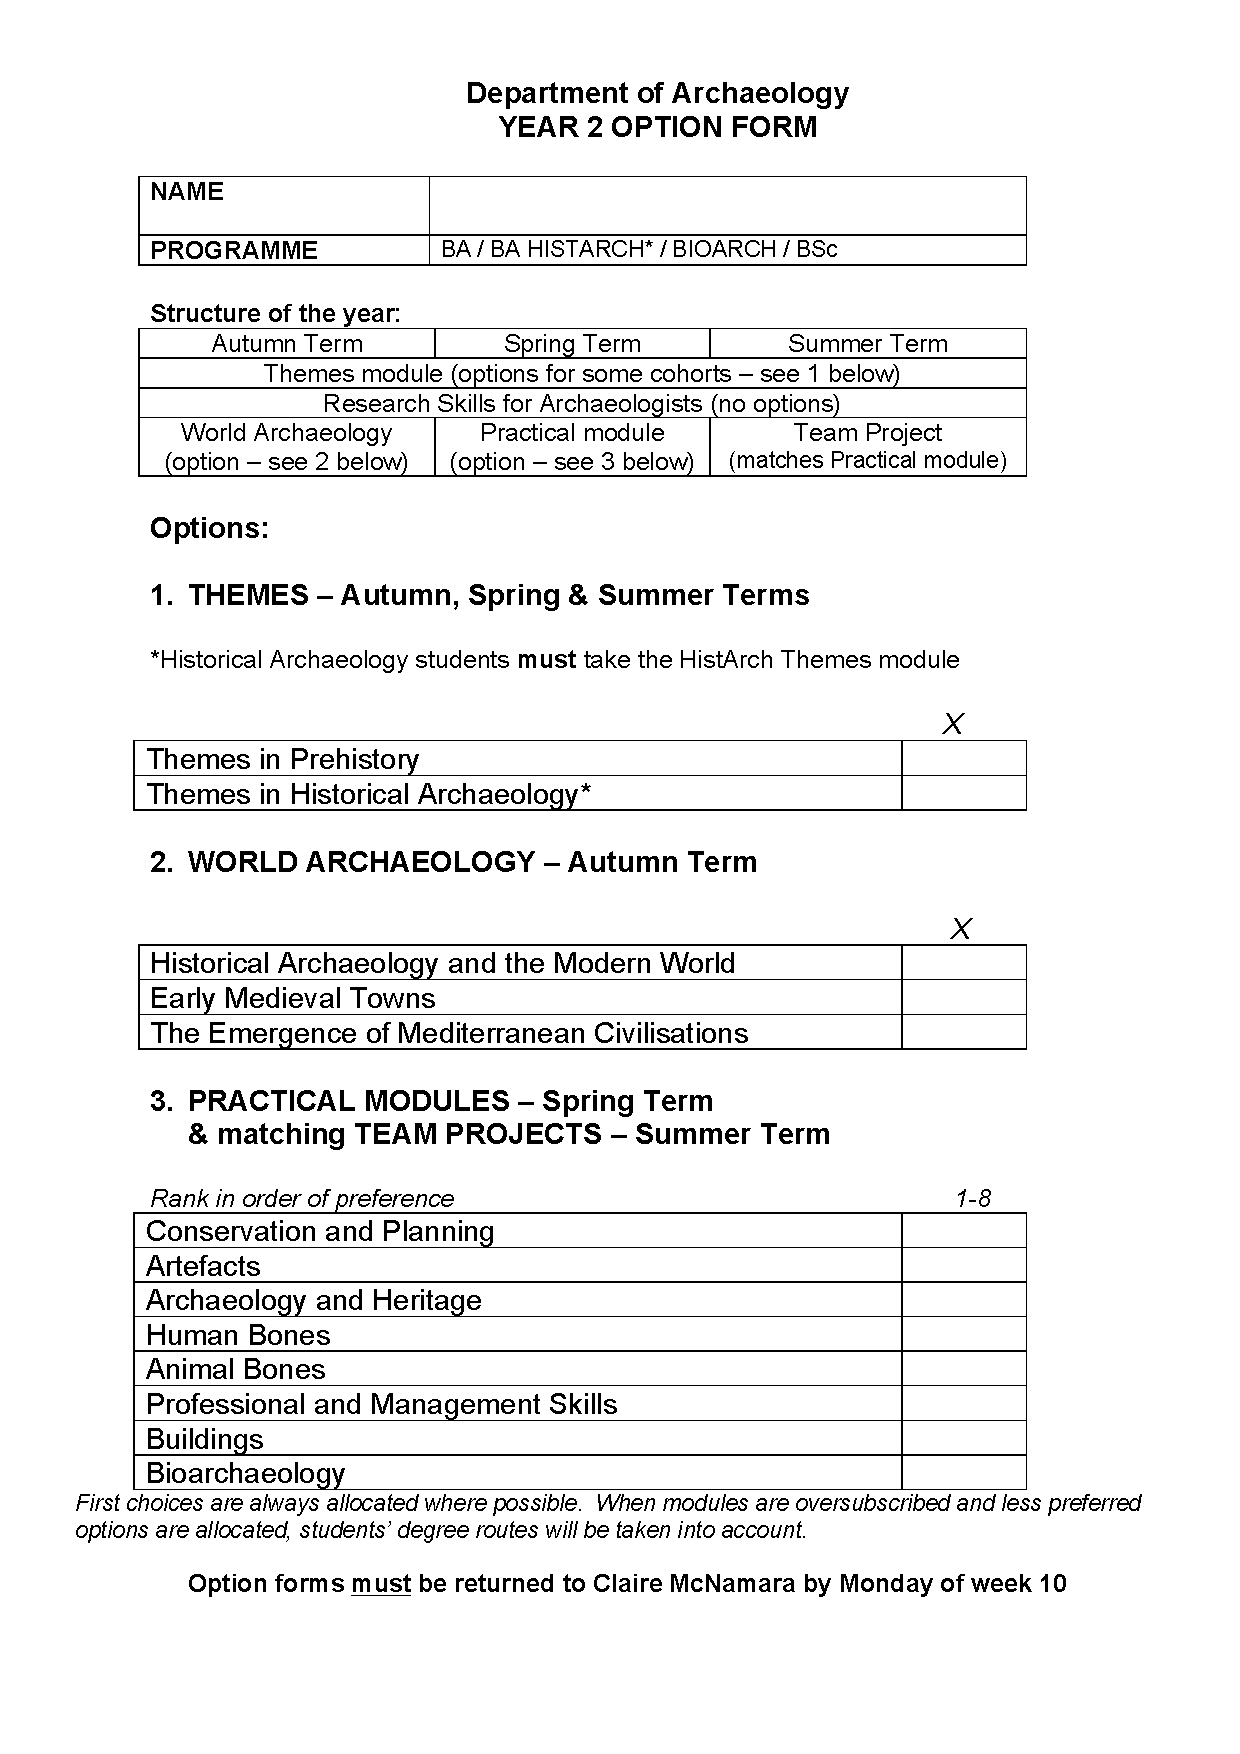
\includegraphics[width=0.9\linewidth]{inc/paperformarchaeology1.pdf}}
      \caption{A paper form given to Archaeology students to select modules}
      \label{paperformarchaeology1}
    \end{minipage}
  \end{figure}
\end{landscape}

\begin{landscape}
  \begin{figure}
    \begin{center}
      \fbox{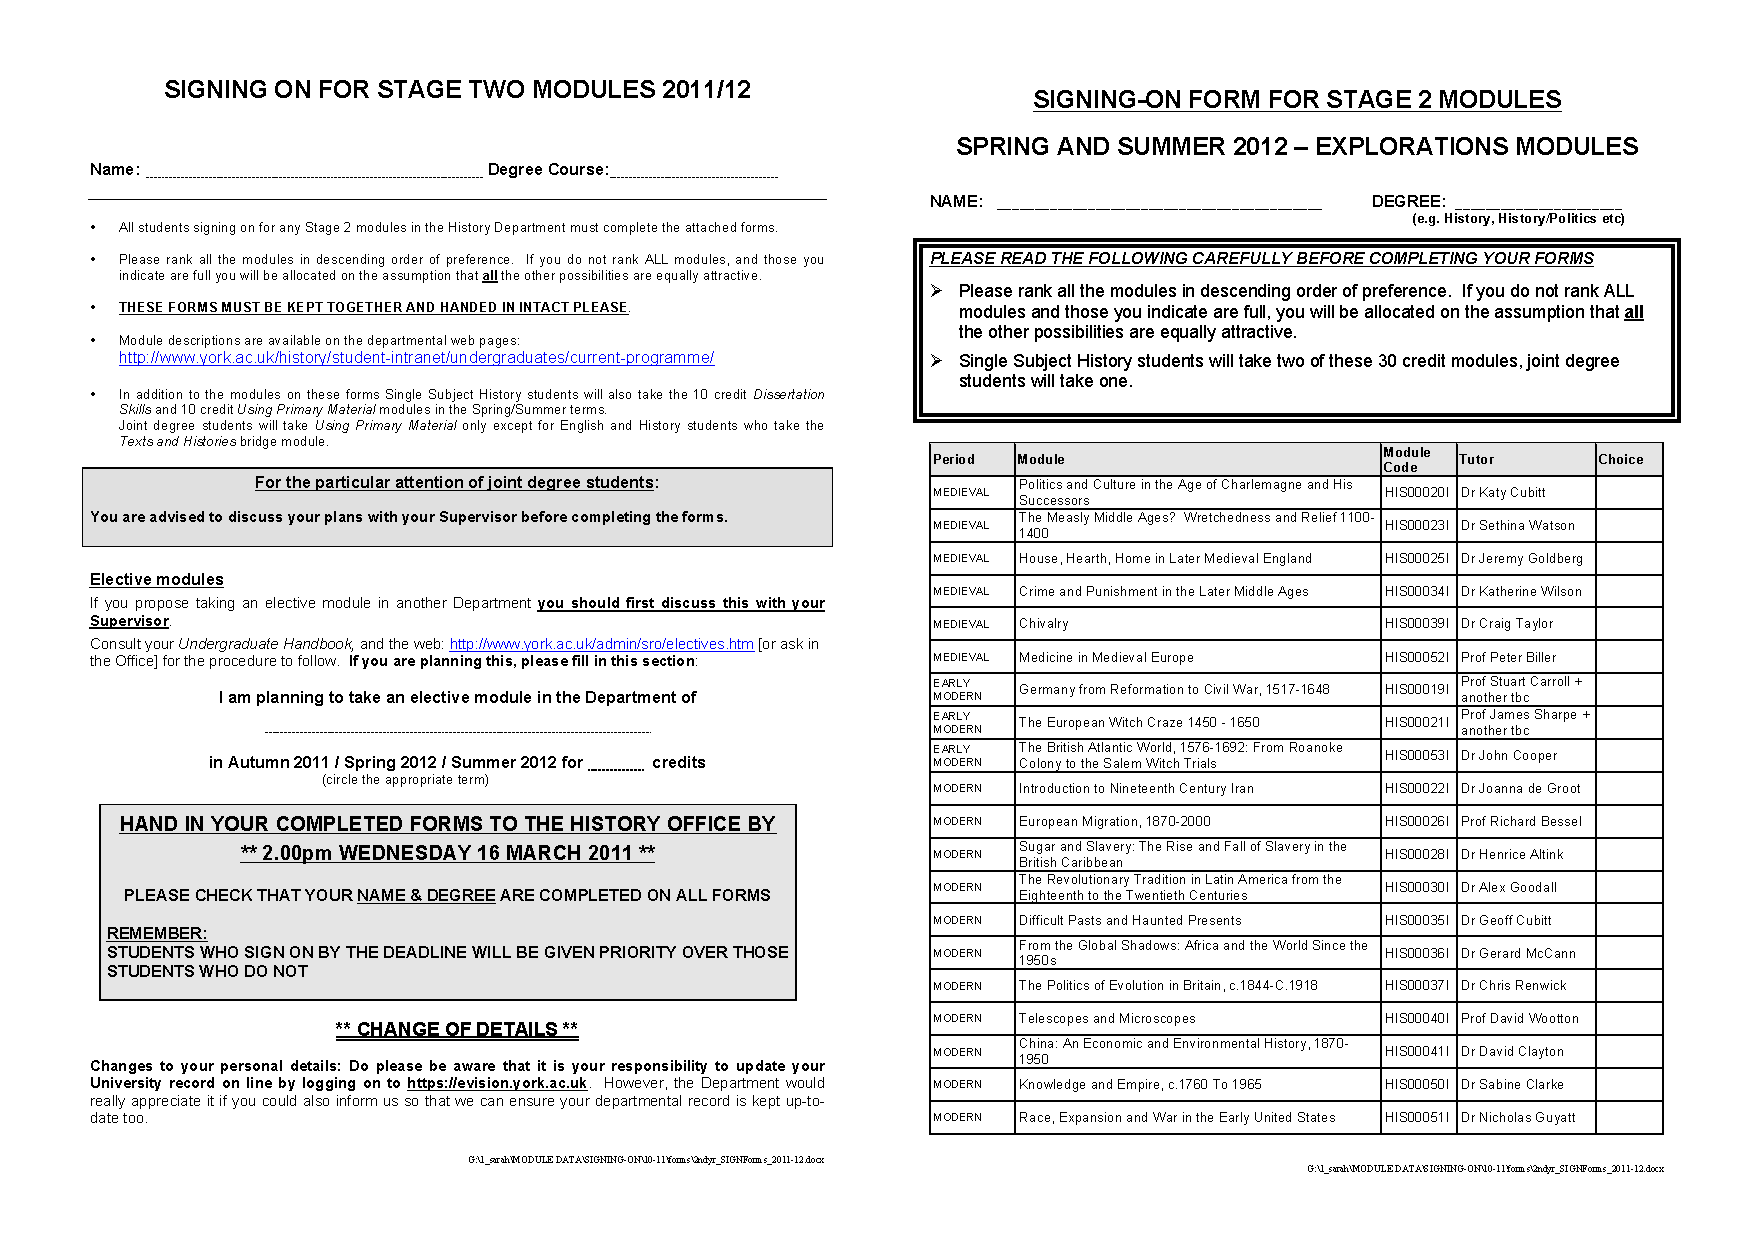
\includegraphics[width=0.9\linewidth]{inc/paperformhistory1.pdf}}
    \end{center}
    \caption{A paper form given to History students to select modules}
    \label{paperformhistory1}
  \end{figure}
\end{landscape}

\stdsection{Prototypes of the student interface}
\label{sec:prototypes}

Figures~\ref{prototype_student_1col}, \ref{prototype_student_weighting} and
\ref{prototype_student_2col} give screenshots of the prototypes created for
the student interface for ranking modules.

Note that the explanatory copy included in the screenshots was drafted
by the project implementer and was revised by the departments prior to the
system being in use.

\begin{figure}
  \begin{center}
    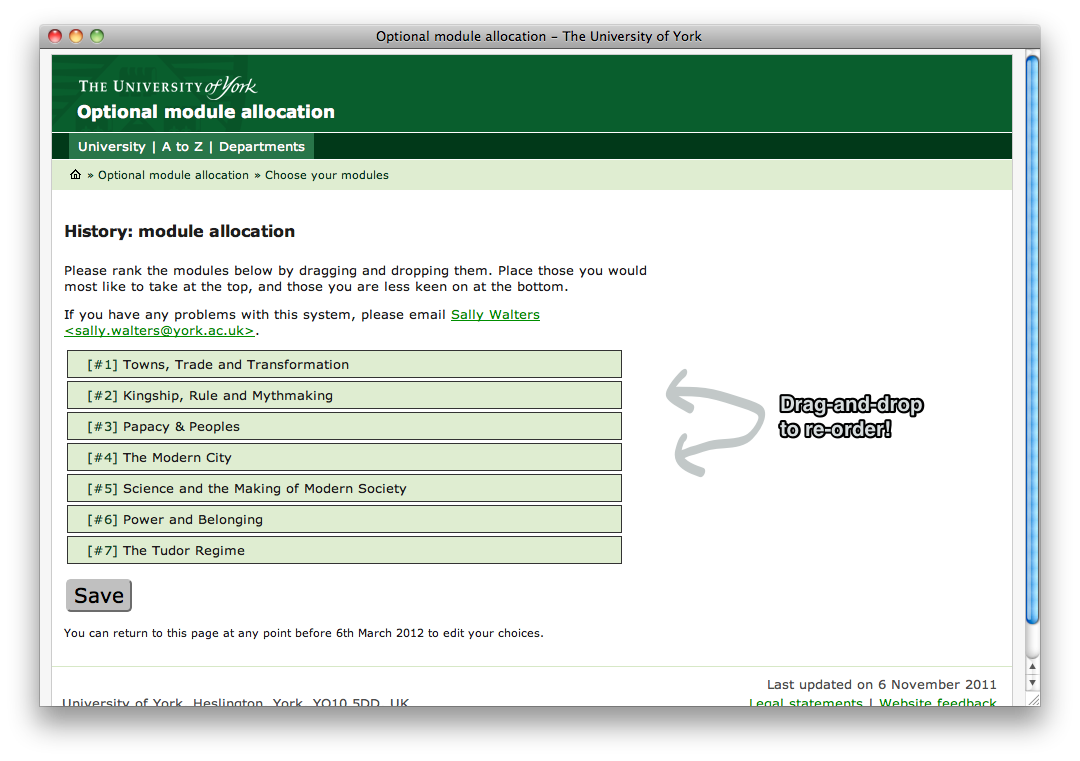
\includegraphics[width=0.85\linewidth]{images/prototypes/student_prototype_1.png}
  \end{center}
  \caption{Prototype of a drag-and-drop ranking based system}
  \label{prototype_student_1col}
\end{figure}

\begin{figure}
  \begin{center}
    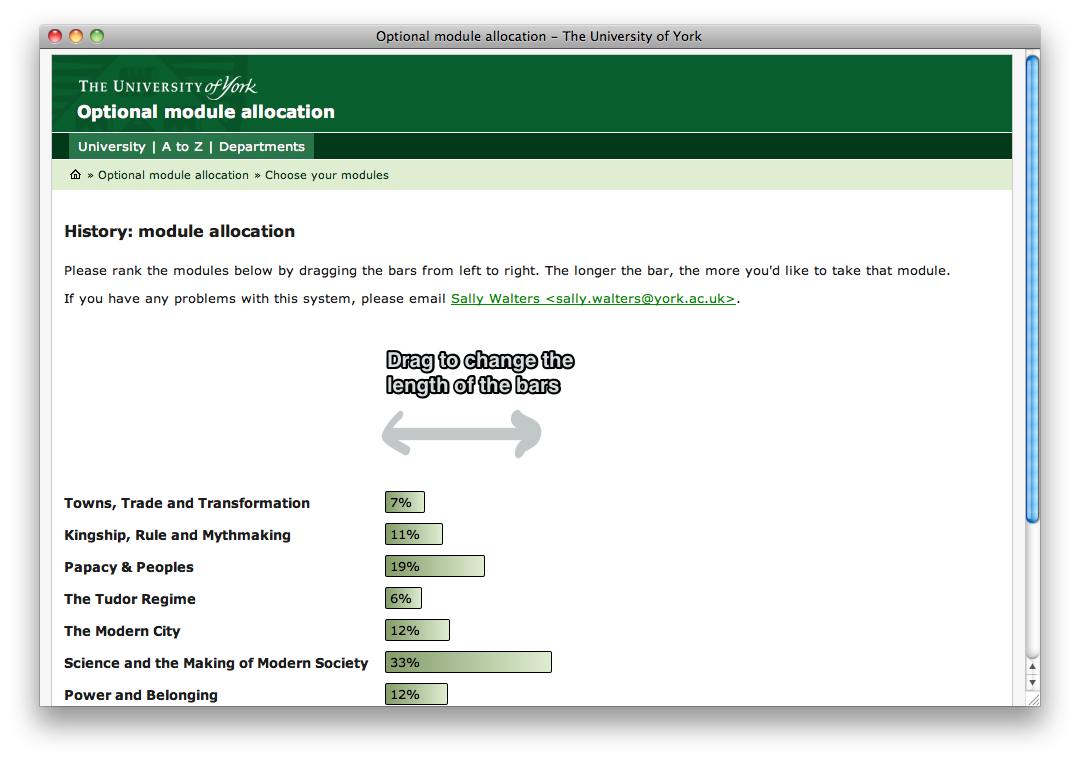
\includegraphics[width=0.85\linewidth]{images/prototypes/student_prototype_2.png}
  \end{center}
  \caption{Prototype of draggable bars for a weighting based system}
  \label{prototype_student_weighting}
\end{figure}

\begin{figure}
  \begin{center}
    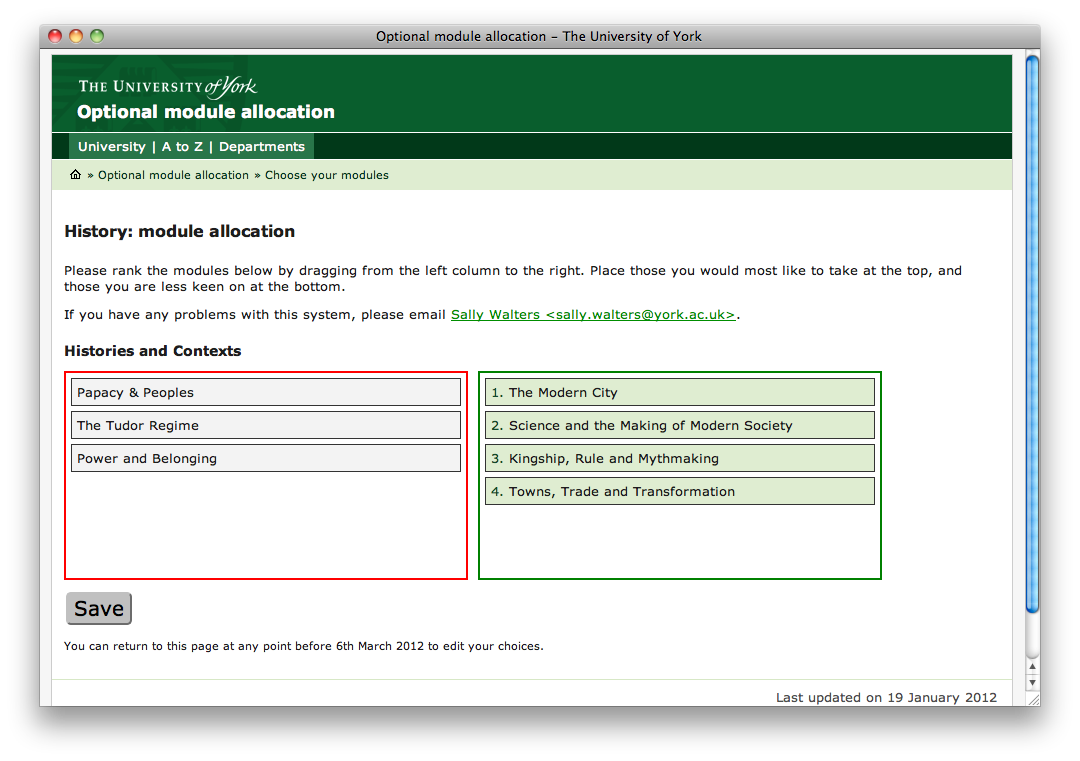
\includegraphics[width=0.85\linewidth]{images/prototypes/student_prototype_3.png}
  \end{center}
  \caption{Prototype of a drag-and-drop two-column ranking based system}
  \label{prototype_student_2col}
\end{figure}

\stdsection{Feedback from test users}
\label{sec:testingfeedback}

\subsection{Focus groups with students}

\begin{itemize}
  \item Students have the expectation that they should have to rank every module
  \item The two-column layout is similar to the way \gls{yusu} voting works
  \item The system should send an email confirmation to students
\end{itemize}

\subsection{Final application on development server}

\begin{itemize}
  \item Form validation improvements (mentioned three times)
  \item Random ordering of modules on confirmation screen (two times)
  \item Parts of explanatory text unclear (two times)
  \item Students should not be required to rank every module (once)
\end{itemize}

\clearpage

\stdsection{Application documentation}
\label{sec:documentation}

The following documentation was provided to every departmental administrator
in advance of the application being open to students (27 February). It was
also used as the basis for the \gls{itservices} security review that is
discussed in Section~\ref{sec:securityreview} (15 February).

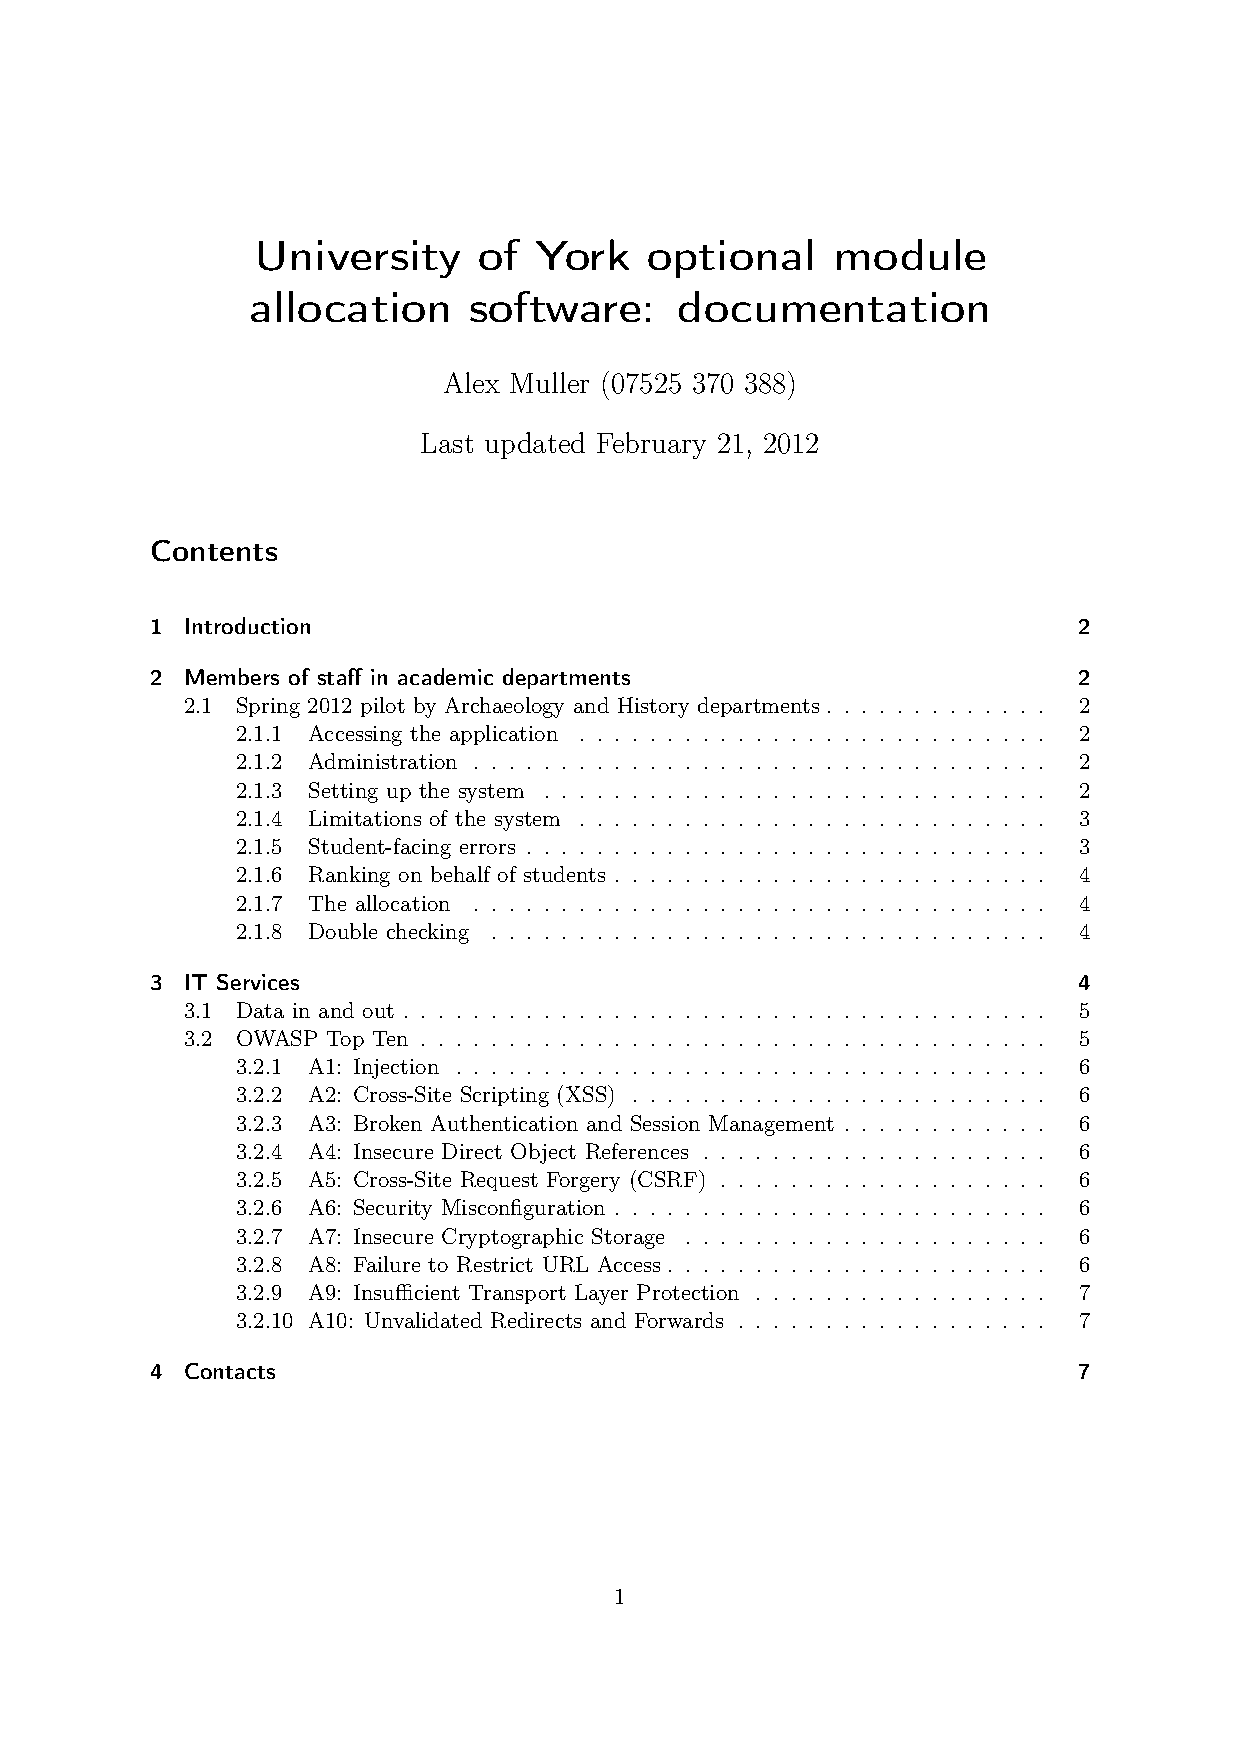
\includepdf[pages=-, frame=true, nup=2, landscape=true]{inc/documentation.pdf}


\begin{landscape}
  \stdsection{Gurobi optimisation code}
  \label{sec:gurobicode}
  
  This appendix contains the code used to allocate the modules to students. Some
  syntax has been modified to fit the constraints of the page and some
  superfluous code has been removed, but otherwise it is unmodified.
  
  \lstset{
    language     = Java,
    multicols    = 2,
    basicstyle   = \ttfamily\tiny,
    keywordstyle = \color{yorkblue}
  }
  \lstinputlisting{listings/AdminAllocate.java}
\end{landscape}

\clearpage
\printglossaries

\clearpage
\bibliographystyle{references/IEEEtran.bst} % not just plain
\bibliography{references/references.bib}
\addcontentsline{toc}{section}{References}


\end{document}
